% Fictitious Play και Reinforcement Learning - Τελική Αναφορά
% Βάση: REPORT.md, εμπλουτισμός: chat_gpt_report.md

\documentclass[11pt,a4paper]{article}

\usepackage[main=greek,english]{babel}
\usepackage{fontspec}
\defaultfontfeatures{Ligatures=TeX}
\setmainfont{Cambria}
\setsansfont{Calibri}
\setmonofont{Consolas}

\usepackage{amsmath,amssymb,amsthm}
\usepackage{graphicx}
\usepackage{grffile}
\usepackage{booktabs}
\usepackage{geometry}
\usepackage{hyperref}
\usepackage{microtype}
\usepackage{ragged2e}
\usepackage{enumitem}
\usepackage{indentfirst}

\geometry{margin=2.5cm}
\linespread{1.15}
\setlength{\parindent}{1.5em}
\setlist{nosep,leftmargin=*}

% Ενιαίο μέγεθος, αποφυγή υπερχείλισης γραμμών
\sloppy
\setlength{\emergencystretch}{2em}

\newcommand{\eng}[1]{\foreignlanguage{english}{#1}}

\title{Fictitious Play και Reinforcement Learning για υπολογισμό ισορροπιών σε μηδενικού αθροίσματος και στοχαστικά παίγνια}
\author{}
\date{Φεβρουάριος 2026}

\begin{document}

\maketitle

\begin{abstract}
Στα πλαίσια της παρούσας εργασίας μελετήσαμε τη συμπεριφορά πρακτόρων σε ανταγωνιστικά περιβάλλοντα. Υλοποιήσαμε και συγκρίναμε δύο βασικές προσεγγίσεις μάθησης: το Fictitious Play (FP), που βασίζεται στη μοντελοποίηση του αντιπάλου μέσω εμπειρικής κατανομής και best response, και το Reinforcement Learning (Q-learning), που μαθαίνει αξίες ενεργειών χωρίς ρητό μοντέλο του αντιπάλου, καθώς και τον αλγόριθμο Minimax για στοχαστικά turn-based παίγνια. Πραγματοποιήσαμε επίσης σύγκριση Minimax και RL στο Grid Hunter-Prey (Hunter με Minimax, Prey με Q-learning). Τα πειράματα διεξήχθησαν σε τρία παίγνια: Matching Pennies, Rock-Paper-Scissors και Grid Hunter-Prey (στοχαστικό, turn-based). Τα πειράματα δείχνουν ότι η έννοια «πλησιάζω Nash» δεν ταυτίζεται με «παίρνω καλύτερο reward» όταν ο αντίπαλος δεν είναι στάσιμος ή όταν και οι δύο μαθαίνουν ταυτόχρονα.
\end{abstract}

\tableofcontents
\newpage

% ========== ΚΕΦΑΛΑΙΟ 1 ==========
\section{Θεωρητικό Πλαίσιο και Στόχοι}

Το θεωρητικό πλαίσιο της εργασίας βασίζεται στο υλικό του μαθήματος «Intelligent Agents and Multiagent Systems» και στις διαφάνειες που παρουσιάζονται κατά τη διάρκεια των μαθημάτων. Ακολουθούμε τη θεωρία που αναπτύχθηκε στο μάθημα για normal-form games, zero-sum παίγνια, Nash equilibrium, repeated games, Fictitious Play και Reinforcement Learning, και την εφαρμόζουμε σε απλά αλλά εκφραστικά παραδείγματα.

Στόχος είναι η κατανόηση σε βάθος και η εφαρμογή χωρίς περιττή πολυπλοκότητα. Τα παραδείγματα επιλέχθηκαν ώστε να φαίνονται ξεκάθαρα τόσο οι δυνατότητες όσο και οι αδυναμίες των αλγορίθμων: η FP συγκλίνει στο Nash αλλά είναι ευάλωτη σε προσαρμοστικούς αντιπάλους· το Q-learning μπορεί να εκμεταλλευτεί προβλεψιμότητα αλλά στο self-play δεν συγκλίνει απαραίτητα σε ισορροπία· η Minimax υπερτερεί όταν το μοντέλο του κόσμου είναι γνωστό.

\subsection{Πράκτορες και Χρησιμότητα}

Οι πράκτορες ορίζονται ως ορθολογικές οντότητες που στοχεύουν στη μεγιστοποίηση της Αναμενόμενης Χρησιμότητας (Maximum Expected Utility, MEU). Κάθε ενέργεια έχει μια συσχέτιση με το αποτέλεσμα και με την πιθανότητα του· ο ορθολογικός πράκτορας επιλέγει εκείνη που μεγιστοποιεί το αναμενόμενο outcome.

Σε περιβάλλοντα πολλαπλών πρακτόρων η χρησιμότητα ενός πράκτορα εξαρτάται όχι μόνο από τις δικές του ενέργειες αλλά και από τις ενέργειες των άλλων. Αυτό οδηγεί σε στρατηγική σκέψη: ο κάθε παίκτης πρέπει να λάβει υπόψη τι μπορεί να κάνει ο άλλος και τι είναι λογικό να περιμένει. Οι έννοιες της θεωρίας παιγνίων (Nash equilibrium, best response, mixed strategies) αναφέρονται ακριβώς σε αυτό το πρόβλημα συντονισμού και ανταγωνισμού.

\subsection{Θεωρία Παιγνίων}

Εστιάζουμε σε παίγνια μηδενικού αθροίσματος (zero-sum), όπου \(U_1 + U_2 = 0\): ό,τι κερδίζει ο ένας χάνει ο άλλος. Σε τέτοια παίγνια ο καθαρός ανταγωνισμός μοντελοποιείται με πίνακες αποδόσεων (payoff matrices). Κάθε γραμμή αντιστοιχεί σε μια ενέργεια του Row Player, κάθε στήλη σε μια ενέργεια του Column Player· το στοιχείο \(M[i,j]\) είναι το payoff του Row όταν παίζουν \((i, j)\).

Σε παίγνιο 2 παικτών σε normal form, ο πίνακας αποδόσεων του Row είναι \(M \in \mathbb{R}^{m \times n}\). Αν ο Row παίξει pure \(i\) και ο Column pure \(j\), ο Row παίρνει \(M_{ij}\) και ο Column παίρνει \(-M_{ij}\). Μικτές στρατηγικές είναι διανύσματα πιθανοτήτων:
\[
x \in \Delta_m = \{x \ge 0,\ \mathbf{1}^\top x = 1\}, \quad
y \in \Delta_n = \{y \ge 0,\ \mathbf{1}^\top y = 1\}.
\]
Το αναμενόμενο payoff του Row είναι:
\[
u(x,y) = x^\top M y.
\]

Η Ισορροπία Nash (NE) είναι το ζεύγος στρατηγικών όπου κανένας παίκτης δεν έχει κίνητρο να αλλάξει μονομερώς: δεδομένης της στρατηγικής του αντιπάλου, η δική του είναι καλύτερη απάντηση (best response). Ένα ζεύγος \((x^*, y^*)\) είναι Nash αν:
\[
x^* \in \arg\max_{x \in \Delta_m} x^\top M y^*, \qquad
y^* \in \arg\min_{y \in \Delta_n} (x^*)^\top M y.
\]
Σε zero-sum, το Nash έχει επίσης καθαρή «ερμηνεία ασφάλειας»: το \(x^*\) μεγιστοποιεί το χειρότερο που μπορεί να του κάνει ο αντίπαλος, και το \(y^*\) ελαχιστοποιεί το καλύτερο που μπορεί να πάρει ο Row.

Στα παίγνια που μελετάμε (Matching Pennies, Rock-Paper-Scissors) δεν υπάρχει Pure Strategy Nash — δεν υπάρχει ζεύγος καθαρών ενεργειών που να είναι αμφίδρομα best response. Υπάρχει όμως μοναδικό Mixed Strategy Nash: και οι δύο παίκτες πρέπει να αναμείνουν τις ενέργειες τους με συγκεκριμένες πιθανότητες (π.χ. 0.5–0.5 στο Matching Pennies, 1/3–1/3–1/3 στο RPS).

\subsubsection{Θεώρημα Minimax και σκιαγράφηση απόδειξης (LP δυϊκότητα)}

Σε zero-sum παίγνια το θεώρημα Minimax εξασφαλίζει ότι η λύση minimax ταυτίζεται με το Nash Equilibrium: η στρατηγική που ελαχιστοποιεί τη μέγιστη ζημιά (maximin) είναι αντίστοιχη με την best response στο NE. Αυτό μας επιτρέπει να χρησιμοποιήσουμε την αναζήτηση Minimax σε sequential games όταν το παίγνιο έχει τέλεια πληροφορία.

Ορίζουμε την τιμή του παιγνίου:
\[
v = \max_{x \in \Delta_m} \min_{y \in \Delta_n} x^\top M y.
\]
Ο Row θέλει να βρει \(x\) που εγγυάται payoff τουλάχιστον \(v\) απέναντι σε κάθε pure δράση του Column. Αυτό γράφεται ως LP· ο Column αντίστοιχα λύνει το δυϊκό LP. Με ισχυρή δυϊκότητα LP έχουμε \(v=w\) στην optimum. Επιπλέον, από συμπληρωματική αδράνεια (complementary slackness) παίρνουμε ότι οι βέλτιστες στρατηγικές \((x^*, y^*)\) ικανοποιούν τις συνθήκες σημείου σέλας:
\[
x^\top M y^* \le (x^*)^\top M y^* \le (x^*)^\top M y, \quad \forall x,y.
\]
Αυτό ακριβώς ισοδυναμεί με Nash ισορροπία σε zero-sum και με την minimax ισότητα:
\[
\max_x \min_y x^\top M y = \min_y \max_x x^\top M y.
\]
Αυτό το κομμάτι είναι ο θεωρητικός «άξονας» των matrix experiments: μας δίνει συγκεκριμένο στόχο (τη mixed Nash) και άρα μετρικές απόστασης από Nash.

\subsection{Μάθηση σε Επαναλαμβανόμενα Παίγνια}

Σε repeated games το ίδιο (stage) παίγνιο παίζεται πολλές φορές. Οι παίκτες μπορούν να μαθαίνουν από το ιστορικό και να προσαρμόζουν τη συμπεριφορά τους. Εξετάζουμε δύο προσεγγίσεις που εμφανίζονται στο μάθημα:

\subsubsection{Model-based: Fictitious Play (FP)}

Ο πράκτορας διατηρεί μια πεποίθηση (belief) για τη στρατηγική του αντιπάλου, βασισμένη στην εμπειρική συχνότητα των κινήσεών του μέχρι τώρα. Σε repeated play, αν ο Column έχει δράσεις \(A\) και μέχρι τον χρόνο \(t\) έχει παίξει την \(a\) για \(w_t(a)\) φορές:
\[
\hat{y}_t(a) = \frac{w_t(a)}{\sum_{a' \in A} w_t(a')}.
\]
Ο Row παίζει best response σε αυτή την πεποίθηση:
\[
i_t \in \arg\max_i \sum_{a \in A} \hat{y}_t(a) \cdot M_{i,a}.
\]
Ο Column κάνει το ανάλογο με πεποίθηση \(\hat{x}_t\) και best response. Σε κάθε γύρο παίζει Best Response (BR) σε αυτό το belief: επιλέγει την ενέργεια που μεγιστοποιεί το αναμενόμενο payoff δεδομένου του belief. Θεωρητικά, σε zero-sum παίγνια η εμπειρική κατανομή και οι best responses συγκλίνουν προς το mixed Nash equilibrium. Η FP είναι ντετερμινιστική δεδομένου του belief — κάθε μικρή αλλαγή στο belief μπορεί να αλλάξει την επιλογή ενέργειας.

Σε παιχνίδια με mixed equilibrium, είναι φυσιολογικό οι καθαρές επιλογές να μην «παγώνουν» σε μία δράση. Το αντικείμενο που έχει νόημα να συγκλίνει είναι οι εμπειρικές κατανομές \((\hat{x}_t, \hat{y}_t)\). Αυτό ταιριάζει με το πώς ορίζεται και η Nash σε mixed στρατηγικές. Ένα χρήσιμο σημείο: η best-response δυναμική μπορεί να παράγει κυκλικότητα σε επίπεδο actions, ακόμη κι όταν οι εμπειρικές συχνότητες πλησιάζουν ισορροπία. Άρα, όταν αξιολογούμε FP, κοιτάμε primarily τις \((\hat{x}_t, \hat{y}_t)\).

\subsubsection{Model-free: Q-Learning}

Ο πράκτορας δεν μοντελοποιεί ρητά τον αντίπαλο. Μαθαίνει τις αξίες (Q-values) των ενεργειών μέσω αλληλεπίδρασης: κάθε φορά που παίζει μια ενέργεια και λαμβάνει reward, ενημερώνει την εκτίμηση της αξίας της. Για state \(s\), action \(a\), reward \(r\), next state \(s'\), η ενημέρωση είναι:
\[
Q(s,a) \leftarrow (1-\alpha) Q(s,a) + \alpha \left[ r + \gamma \max_{a'} Q(s',a') \right].
\]
Η ενημέρωση βασίζεται στην εξίσωση Bellman (σε stochastic MDPs· στα απλά matrix games η αξία είναι άμεσα το αναμενόμενο reward). Η πολιτική επιλογής δράσης είναι συνήθως \(\varepsilon\)-greedy:
\[
a = \begin{cases} \text{random action}, & \text{με πιθανότητα } \varepsilon \\
\arg\max_a Q(s,a), & \text{με πιθανότητα } 1-\varepsilon. \end{cases}
\]
Αυτό εξισορροπεί exploration–exploitation και επιτρέπει τη μάθηση χωρίς model του αντιπάλου.

Σε MDP το transition kernel και τα rewards είναι στάσιμα. Σε multiagent, αυτό που «βλέπει» ο ένας παίκτης εξαρτάται από την πολιτική του άλλου. Αν η πολιτική του άλλου αλλάζει, τότε το effective περιβάλλον γίνεται μη-στάσιμο. Αυτό σημαίνει ότι η σύγκλιση του tabular Q-learning σε μία fixed optimal Q δεν είναι κάτι που πρέπει να θεωρείται δεδομένο σε self-play. Έτσι, στα matrix games το Q-learning τείνει να μάθει «πώς να παίρνει reward απέναντι στον συγκεκριμένο αντίπαλο/στο συγκεκριμένο training dynamics», όχι «πώς να παίζει Nash». Ωστόσο, σε non-stationary περιβάλλοντα (όπου ο αντίπαλος αλλάζει συνεχώς) οι υποθέσεις σύγκλισης του Q-learning δεν ισχύουν.

Στο stochastic/turn-based παιχνίδι Grid Hunter-Prey ως Markov game: το state είναι \(s = (\mathrm{pos}_H, \mathrm{pos}_P)\) και οι πράξεις του Hunter/Prey αλλάζουν την κατάσταση. Η στόχευση είναι long-horizon: ο Hunter θέλει να μεγιστοποιήσει πιθανότητα και ταχύτητα σύλληψης, το Prey να μεγιστοποιήσει διαφυγή/timeout. Το Q-learning είναι εδώ φυσική επιλογή επειδή μαθαίνει state-dependent πολιτικές.

\subsection{Μετρικές Απόδοσης και No-Regret}

Για την αξιολόγηση χρησιμοποιούμε τις ακόλουθες μετρικές, οι οποίες αναφέρονται στη θεωρία repeated games:

\begin{itemize}
\item Απόσταση από το Nash (distance to Nash): Ευκλείδεια (L2) απόσταση της τρέχουσας μικτής στρατηγικής από το θεωρητικό NE. Μικρή τιμή σημαίνει ότι ο πράκτορας έχει συγκλίνει κοντά στην ισορροπία.

\item Cumulative reward: Το άθροισμα των rewards σε όλους τους γύρους. Σε zero-sum είναι αντισυμμετρικό ανά ζεύγος πρακτόρων.

\item External regret: Η διαφορά ανάμεσα στο κέρδος που θα είχε ο πράκτορας αν είχε παίξει πάντα την καλύτερη σταθερή ενέργεια (best fixed action in hindsight) έναντι του πραγματικού ιστορικού του αντιπάλου, μείον το πραγματικό συνολικό κέρδος του. Θετικό regret = «θα είχα κερδίσει περισσότερα με διαφορετική στρατηγική».

\item Exploitability: Πόσο μπορεί να κερδίσει ένας εξωτερικός παίκτης παίζοντας best response απέναντι στη τρέχουσα στρατηγική. Υψηλή exploitability = η στρατηγική είναι εύκολα εκμεταλλεύσιμη.
\end{itemize}

Οι αλγόριθμοι no-regret (Hannan consistent) έχουν sublinear external regret (\(O(\sqrt{T})\) ή καλύτερο). Η θεωρία συνδέει τη no-regret ιδιότητα με τη σύγκλιση σε correlated/coarse correlated equilibria σε repeated games. Στα πειράματά μας η FP δεν είναι no-regret απέναντι σε προσαρμοστικούς αντιπάλους· το external regret της FP αυξάνεται γραμμικά όταν αντιμετωπίζει RL.

% ========== ΚΕΦΑΛΑΙΟ 2 ==========
\section{Αρχιτεκτονική Συστήματος και Ανάλυση Υλοποίησης}

Αυτή η ενότητα περιγράφει λεπτομερώς την υλοποίηση ώστε ο αναγνώστης να κατανοήσει τη ροή των αλγορίθμων, τη λογική τους, τις εσωτερικές δομές δεδομένων και τη σύνδεσή τους με τη θεωρία χωρίς να χρειάζεται να ανοίξει τον κώδικα. Κάθε υποενότητα εξηγεί τι συμβαίνει βήμα-βήμα, γιατί τα πράγματα γίνονται με τον τρόπο που γίνονται και σε ποια αρχεία αντιστοιχεί η λογική. Η θεωρία του Κεφαλαίου 1 αποτελεί τη βάση για όλες τις επιλογές σχεδίασης.

\subsection{Γενική Αρχιτεκτονική και Διαχωρισμός Ευθυνών}

Η υλοποίηση είναι αρθρωτή σε Python με τρία επίπεδα αφαίρεσης:

\begin{enumerate}
\item Παιγνία (\eng{games/}): Ορίζουν τους κανόνες, τους πίνακες αποδόσεων και τη δυνατότητα υπολογισμού Nash equilibrium. Δεν περιέχουν λογική πρακτόρων.

\item Πράκτορες (\eng{agents/}): Υλοποιούν τις στρατηγικές μάθησης (FP, Q-learning, Minimax). Κάθε πράκτορας έχει εσωτερική κατάσταση και ακολουθεί το κύκλο: act → receive payoff/state → update.

\item Πειράματα και Ανάλυση (\eng{experiments/}, \eng{analysis/}): Τρέχουν τα σεναρία, συλλέγουν δεδομένα και υπολογίζουν τις μετρικές αξιολόγησης.
\end{enumerate}

Όλοι οι πράκτορες υλοποιούν την ίδια διεπαφή (act, update, get\_strategy, reset), ώστε να μπορούν να συνδυαστούν ελεύθερα σε οποιοδήποτε παίγνιο που το υποστηρίζει.

\subsection{Πλαίσιο Παιγνίων (\eng{games/})}

\subsubsection{BaseGame και matrix games (\eng{base\_game.py}, \eng{matching\_pennies.py}, \eng{rps.py})}

Η κλάση \eng{BaseGame} ορίζει την αφηρημένη διεπαφή για zero-sum παίγνια σε normal-form. Κεντρικό στοιχείο είναι ο πίνακας αποδόσεων (payoff matrix): \(M[i][j]\) = το payoff του Row Player όταν παίζει την ενέργεια \(i\) και ο Column Player την ενέργεια \(j\). Λόγω zero-sum, ο Column Player λαμβάνει \(-M[i][j]\).

Η μέθοδος \eng{get\_payoff(action1, action2)} επιστρέφει άμεσα το στοιχείο του πίνακα για το ζεύγος ενεργειών.

Η μέθοδος \eng{best\_response(opponent\_strategy, player\_id)} είναι κρίσιμη και αξίζει διευκρίνισης. Δέχεται μια μικτή στρατηγική του αντιπάλου (διανυσμα πιθανοτήτων π.χ. [0.3, 0.7]). Για τον Row Player (player\_id=0): υπολογίζει το αναμενόμενο payoff κάθε δικής του ενέργειας ως \(M \cdot \textit{opponent\_strategy}\) (γραμμικός συνδυασμός των στηλών βάσει των πιθανοτήτων του αντιπάλου) και επιστρέφει το argmax — δηλαδή τη καθαρή στρατηγική που μεγιστοποιεί το αναμενόμενο κέρδος. Για τον Column Player (player\_id=1): υπολογίζει \(M^\top \cdot \textit{opponent\_strategy}\) (όπου opponent\_strategy είναι η στρατηγική του Row) και επιστρέφει το argmin, αφού ο Column Player ελαχιστοποιεί το payoff του Row.

\eng{MatchingPennies} (\eng{matching\_pennies.py}): Πίνακας 2×2. Heads=0, Tails=1. Η γραμμή [1,−1] αντιστοιχεί σε Heads: κερδίζεις +1 αν ο αντίπαλος παίξει Heads, −1 αν Tails. Το Nash equilibrium είναι (0.5, 0.5) — και οι δύο παίκτες πρέπει να μπερδεύουν το αντίπαλο παίζοντας 50–50.

\eng{Rock-Paper-Scissors} (\eng{rps.py}): Πίνακας 3×3. Rock=0, Paper=1, Scissors=2. Νίκη +1, ήττα −1, ισοπαλία 0. Το Nash είναι (1/3, 1/3, 1/3).

\subsubsection{Grid Game (\eng{grid\_game.py}) — Στοχαστικό turn-based παίγνιο}

Το \eng{GridGame} δεν είναι normal-form παίγνιο· είναι sequential με καταστάσεις και δεν κληρονομεί από BaseGame. Πλέγμα 3×3, Hunter vs Prey, εναλλασσόμενες κινήσεις (Hunter κινείται πρώτος ή Prey, ανάλογα με την παράμετρο first\_player).

Κατάσταση: Τέσσερις συντεταγμένες (hunter\_row, hunter\_col, prey\_row, prey\_col) που «ισιώνονται» σε ένα αριθμό 0–80 για ευκολία στην Q-table.

Ενέργειες: 0=Up, 1=Right, 2=Down, 3=Left, 4=Stay. Οι κινήσεις ορίζονται με dictionary· κάθε κίνηση εφαρμόζεται με boundary checks ώστε το token να μένει μέσα στο πλέγμα.

Rewards: Capture (Hunter πέφτει πάνω στο Prey): +10 Hunter, −10 Prey. Timeout (max\_steps=20 χωρίς capture): −10 Hunter, +10 Prey. Σε μη-τελικές κινήσεις χρησιμοποιείται distance-based shaping: η διαφορά Manhattan distance πριν και μετά την κίνηση δίνει ένα μικρό πρόσθετο reward (π.χ. πλησίασμα → θετικό για Hunter), ώστε να βοηθεί η μάθηση χωρίς να αλλάζει το βέλτιστο outcome.

Η μέθοδος \eng{step(action)} εκτελεί τη κίνηση του τρέχοντος παίκτη, ενημερώνει τις θέσεις και επιστρέφει (reward, done, next\_player). Η \eng{clone()} αντίγραφα του παιγνίου χρειάζονται για το Minimax, που κάνει προσομοίωση συνεχόμενων κινήσεων χωρίς να αλλάζει το πραγματικό game state.

\subsection{Πλαίσιο Πρακτόρων (\eng{agents/})}

Όλοι οι πράκτορες κληρονομούν από \eng{BaseAgent} (\eng{base\_agent.py}), που ορίζει:

\begin{itemize}
\item \eng{act(game)}: Επιστρέφει δείκτη ενέργειας (0 έως n\_actions−1).
\item \eng{update(action, reward, opponent\_action)}: Ενημερώνει την εσωτερική κατάσταση μετά το round.
\item \eng{get\_strategy()}: Επιστρέφει την τρέχουσα μικτή στρατηγική (πιθανότητες ανά ενέργεια) — χρειάζεται για τις μετρικές (απόσταση Nash, exploitability).
\item \eng{reset()}: Μηδενίζει την κατάσταση για νέο πείραμα.
\end{itemize}

Κάθε πράκτορας διατηρεί \eng{action\_history} και \eng{reward\_history} για μετρικές και visualization.

\subsubsection{Fictitious Play (\eng{fictitious\_play.py})}

Εσωτερική κατάσταση:

\begin{itemize}
\item \eng{opponent\_history}: Λίστα με όλες τις ενέργειες που έπαιξε ο αντίπαλος μέχρι τώρα.
\item \eng{action\_counts}: Πίνακας μήκους n\_actions· action\_counts[a] = πόσες φορές ο αντίπαλος έπαιξε την ενέργεια a.
\item \eng{belief}: Η τρέχουσα πεποίθηση για τη στρατηγική του αντιπάλου — ισοδύναμη με την εμπειρική συχνότητα των κινήσεών του.
\end{itemize}

Αρχικοποίηση: belief = ομοιόμορφη κατανομή (1/n\_actions για κάθε ενέργεια)· action\_counts = μηδενικά.

\eng{act()}: Καλεί \eng{game.best\_response(self.belief, self.player\_id)}. Δηλαδή: δεδομένης της πεποίθησης για τον αντίπαλο, επιλέγει την καθαρή ενέργεια που μεγιστοποιεί (Row) ή ελαχιστοποιεί (Column) το αναμενόμενο payoff. Δεν υπάρχει τυχαιότητα — η FP είναι ντετερμινιστική με δεδομένο το belief.

\eng{update()}: Μόλις ο αντίπαλος παίξει, προστίθεται η ενέργειά του στο opponent\_history. Το action\_counts[opponent\_action] αυξάνεται κατά 1. Το belief υπολογίζεται ως action\_counts / total\_actions, δηλαδή η αναλογία κάθε ενέργειας στο σύνολο των γύρων. Αυτή η αριθμητικά σταθερή αναλυτική ενημέρωση (\(O(1)\) ανά γύρο) είναι ισοδύναμη με το να υπολογίζουμε ξανά τις εμπειρικές συχνότητες από το opponent\_history.

Σύνδεση με τη θεωρία: Η εμπειρική συχνότητα συγκλίνει θεωρητικά στο Nash σε zero-sum games (Robinson). Η best response στο belief οδηγεί τη δική μας στρατηγική προς το NE. Ωστόσο, η FP παίζει ντετερμινιστικά best response — όποτε το belief αλλάζει ελαφρώς, αλλάζει και η ενέργεια. Ένας προσαρμοστικός αντίπαλος (π.χ. RL) μπορεί να εντοπίσει αυτό το pattern και να το εκμεταλλευτεί.

\subsubsection{Q-Learning για matrix games (\eng{q\_learning.py})}

Εσωτερική κατάσταση:

\begin{itemize}
\item \eng{Q}: Πίνακας μήκους n\_actions. Q[a] = εκτιμώμενη αξία της ενέργειας a. Στα matrix games δεν υπάρχουν καταστάσεις — οι Q-values είναι ανά ενέργεια μόνο.
\item \eng{learning\_rate} (\(\alpha\)), \eng{epsilon} (\(\varepsilon\)): με optional decay.
\end{itemize}

Αρχικοποίηση: Q = μηδενικά, \(\varepsilon\) = 0.1 (10\% exploration).

\eng{act()} — epsilon-greedy: Με πιθανότητα \(\varepsilon\) επιλέγει τυχαία ενέργεια. Με πιθανότητα \(1-\varepsilon\) επιλέγει το argmax των Q-values. Σε ισοπαλία (περισσότερες ενέργειες με το ίδιο max Q) επιλέγεται τυχαία μία από αυτές.

\eng{update()}: Μόλις παίξει την ενέργεια a και λάβει reward r:
\(Q[a] = Q[a] + \alpha \cdot (r - Q[a])\).
Αυτή είναι η απλή ενημέρωση δίχως Bellman (γιατί δεν υπάρχουν καταστάσεις)· το reward θεωρείται άμεση ανταμοιβή. Παράλληλα εφαρμόζεται decay στα \(\varepsilon\) και \(\alpha\) (αν ενεργό)· π.χ. epsilon = max(min\_epsilon, epsilon * epsilon\_decay).

\eng{get\_strategy()}: Για τις μετρικές χρειάζουμε μικτή στρατηγική. Η Q-learning δεν διατηρεί ρητή κατανομή· προσεγγίζουμε: κάθε ενέργεια παίρνει πιθανότητα \(\varepsilon\)/n\_actions από το exploration, και οι best actions (argmax Q) μοιράζονται το υπόλοιπο \((1-\varepsilon)\) ισομερώς.

Σύνδεση με τη θεωρία: Το Q-learning είναι model-free· δεν μοντελοποιεί τον αντίπαλο. Μαθαίνει από τα rewards που λαμβάνει. Σε stationary περιβάλλον (σταθερός αντίπαλος) το Q(a) συγκλίνει στην αναμενόμενη αξία της ενέργειας a. Σε non-stationary περιβάλλον (ο αντίπαλος αλλάζει συνεχώς, π.χ. άλλος Q-learning agent) οι υποθέσεις σύγκλισης δεν ισχύουν και η δυναμική μπορεί να είναι κυκλική ή ασταθής. Αντίθετα, απέναντι σε FP που είναι προβλέψιμη, το RL μπορεί να «βλέπει» τα μικρά patterns και να τα εκμεταλλεύεται.

\subsubsection{Stochastic Q-Learning για grid game (\eng{stochastic\_q\_learning.py})}

Διαφορά από το απλό Q-learning: Υπάρχουν καταστάσεις. \(Q(s, a)\) = εκτιμώμενη συνολική ανταμοιβή αν ξεκινήσουμε από s, παίξουμε a και ακολουθήσουμε βέλτιστα μετά.

Εσωτερική κατάσταση:

\begin{itemize}
\item \eng{Q}: Λεξικό (ή πίνακας) state → array of Q-values. Για 81 καταστάσεις (3×3×3×3) και 5 ενέργειες: Q[state] έχει μήκος 5.
\item \eng{last\_state}: Η τελευταία κατάσταση από την οποία πράξαμε (χρειάζεται για την ενημέρωση).
\item \eng{gamma} (\(\gamma\)): Παράγοντας έκπτωσης.
\end{itemize}

\eng{act(game, state)}: Αν state δεν δίνεται, λαμβάνεται από game.get\_state(). Εφαρμόζεται epsilon-greedy πάνω στο Q[state].

\eng{update(action, reward, next\_state, done)}: Αν η κατάσταση είναι τελική (done=True): target = reward. Αλλιώς: target = reward + \(\gamma\) * max\_a' Q(next\_state, a') — κλασική Bellman ενημέρωση. Τότε:
\(Q[s][a] \leftarrow Q[s][a] + \alpha \cdot (\mathrm{target} - Q[s][a])\).
Το epsilon και το \(\alpha\) μειώνονται με decay ώστε να περνάμε από exploration σε exploitation.

Σύνδεση με τη θεωρία: Η Bellman equation ορίζει την βέλτιστη αξία· η Q-learning ενημέρωση είναι sample-based προσέγγιση. Το \(\gamma<1\) δίνει έμφαση σε βραχυπρόθεσμα rewards· το distance shaping βοηθά τη σύγκλιση χωρίς να αλλοιώνει το τελικό objective.

\subsubsection{Minimax (\eng{minimax.py})}

Χρήση: Μόνο στο Grid Game, ως Hunter. Απαιτεί τέλεια γνώση του παιγνίου (κανόνες, transitions)· δεν μαθαίνει.

Εσωτερική κατάσταση: Βάθος αναζήτησης (depth) και προαιρετική evaluation function για μη-τελικές καταστάσεις.

\eng{act(game)}: Για κάθε δυνατή κίνηση, κλωνοποιεί το παίγνιο, εκτελεί την κίνηση και αν το παίγνιο τελειώνει αξιολογεί το αποτέλεσμα· αλλιώς καλεί αναδρομικά \_minimax με μειωμένο βάθος. Ο Hunter μεγιστοποιεί· ο Prey (εναλλαγή σειράς στο minimax tree) ελαχιστοποιεί. Επιστρέφει την ενέργεια με το καλύτερο αξιολογικό αποτέλεσμα.

\eng{\_minimax(game, depth, is\_maximizing)}: Αν depth=0, επιστρέφει \_evaluate(game). Αλλιώς: αν is\_maximizing, δοκιμάζει όλες τις κινήσεις και κρατά το max· αλλιώς το min. Χρησιμοποιείται evaluation function βασισμένη στην απόσταση Hunter–Prey (ή custom function αν παρέχεται).

\eng{update()}: Απλά καταγράφει action και reward (για συμβατότητα με το runner)· δεν αλλάζει τη συμπεριφορά.

Σύνδεση με τη θεωρία: Το θεώρημα Minimax εξασφαλίζει βέλτιστη παιξιά σε παίγνια με τέλεια πληροφορία. Όταν το μοντέλο είναι γνωστό, η αναζήτηση δίνει άμεσο πλεονέκτημα έναντι learning.

\subsection{Ροή Πειραμάτων (\eng{experiments/runner.py})}

Ο \eng{ExperimentRunner} ανιχνεύει αυτόματα τον τύπο παιγνίου:

\begin{itemize}
\item Matrix game: Έχει get\_payoff και get\_nash\_equilibrium. Simultaneous play.
\item Turn-based: Έχει step, get\_current\_player, reset. Sequential play.
\end{itemize}

Για matrix games (Matching Pennies, RPS), κάθε iteration:

\begin{enumerate}
\item Καλούνται ταυτόχρονα agent1.act(game) και agent2.act(game).
\item Υπολογίζονται τα payoffs: payoff1 = game.get\_payoff(a1, a2), payoff2 = −payoff1 (zero-sum).
\item Καλούνται agent1.update(a1, payoff1, a2) και agent2.update(a2, payoff2, a1) — τώρα κάθε πράκτορας γνωρίζει και την ενέργεια του αντιπάλου.
\item Καθώς και τα δύο agents έχουν ενημερωθεί, καλούνται get\_strategy() και υπολογίζονται: distance\_to\_nash για κάθε πράκτορα, exploitability, και αποθηκεύονται strategy\_history, reward\_history, action\_history.
\end{enumerate}

Για turn-based games (Grid):

\begin{enumerate}
\item Καθορίζεται ο current\_player (Hunter ή Prey).
\item Ο αντίστοιχος πράκτορας καλεί act(game, state).
\item Εκτελείται game.step(action)· επιστρέφει (reward, done, next\_player).
\item Ο πράκτορας ενημερώνεται με update(..., next\_state=..., done=...). Για StochasticQLearning χρειάζεται το next\_state και το done για τη Bellman ενημέρωση.
\item Αν done=True, το παίγνιο κάνει reset και ξεκινά νέο episode.
\item Τα rewards καταγράφονται ανά πράκτορα (0 όταν δεν κάνει κίνηση ο άλλος).
\end{enumerate}

Τα scripts \eng{fp\_vs\_fp.py}, \eng{fp\_vs\_rl.py}, \eng{rl\_vs\_rl.py} δημιουργούν τα κατάλληλα agents και game, τρέχουν τον ExperimentRunner, και παράγουν plots και results.txt μέσω του visualizer.

\subsection{Μετρικές και Αξιολόγηση (\eng{analysis/metrics.py})}

\begin{itemize}
\item \eng{distance\_to\_nash(strategy, nash)}: Ευκλείδεια (L2) απόσταση του διανύσματος στρατηγικής από το θεωρητικό Nash. Μικρή τιμή = κοντά σε ισορροπία.

\item \eng{exploitability(strategy, game, player\_id)}: Υπολογίζει πόσο μπορεί να κερδίσει ο \emph{αντίπαλος} παίζοντας best response απέναντι στη στρατηγική μας. Χρησιμοποιείται το best response του αντιπάλου (όχι του παίκτη που αξιολογείται). Μεγάλη exploitability = η στρατηγική είναι εύκολα εκμεταλλεύσιμη· μηδέν στο Nash.

\item \eng{external\_regret(agent\_history, opponent\_history, game, player\_id)}: Για κάθε χρονική στιγμή t, υπολογίζει το payoff που θα είχε ο πράκτορας αν είχε παίξει πάντα την ίδια (best fixed) ενέργεια έναντι του ιστορικού του αντιπάλου. Το regret = best\_fixed\_reward − actual\_reward. Θετικό = θα είχε κερδίσει περισσότερο με σταθερή στρατηγική.

\item \eng{external\_regret\_history}: Ίδια λογική αλλά επιστρέφει λίστα regret ανά t για plotting.

\item \eng{convergence\_speed(strategy\_history, nash, threshold)}: Επιστρέφει την πρώτη iteration όπου η απόσταση από το Nash πέφτει κάτω από το threshold.

\item \eng{cumulative\_reward}, \eng{average\_payoff}: Αθροιστικό και μέσο reward.
\end{itemize}

Ο visualizer χρησιμοποιεί αυτές τις μετρικές για γραφήματα εξέλιξης στρατηγικής, distance to Nash, cumulative reward, exploitability heatmap κ.λπ., τα οποία αποθηκεύονται σε \eng{results/plots/\{game\}/\{agent\_combo\}/}.

\subsection{Σύστημα Ανταμοιβών και Παράμετροι}

Matrix games: Matching Pennies και RPS έχουν συμμετρικά payoffs (+1/−1 ή 0) ώστε \(R_1+R_2=0\). Η σύγκριση με το θεωρητικό NE είναι άμεση.

Grid Game: Capture +10/−10, timeout −10/+10, distance shaping σε μη-τελικές κινήσεις. Ο \(\gamma=0.99\) δίνει έμφαση σε μακροπρόθεσμα outcomes.

Παράμετροι πειραμάτων: Για matrix: 10.000 iterations, \(\alpha=0.1\), \(\varepsilon=0.1\), seed=42. Για grid: 200.000 turns, Minimax depth=4, \(\gamma=0.99\), epsilon decay. Επιλέχθηκαν ώστε να φανούν σύγκλιση FP, εκμετάλλευση FP από RL και αστάθεια RL vs RL.

% ========== ΚΕΦΑΛΑΙΟ 3 ==========
\section{Πειραματική Ανάλυση και Αποτελέσματα}

Τα τρία παίγνια και τα επτά σεναρία πειραμάτων παρέχουν έναν πλούσιο πίνακα αποτελεσμάτων. Τα δεδομένα προέρχονται από τα αρχεία \eng{results/plots/\{game\}/\{scenario\}/results.txt}. Παρακάτω παρουσιάζονται με λεπτομέρεια και σύγκριση μεταξύ σεναρίων.

\subsection{Σύνοψη αποτελεσμάτων}

\begin{center}
\small
\resizebox{\textwidth}{!}{%
\begin{tabular}{@{}llccp{3.8cm}@{}}
\toprule
Παίγνιο & Σενάριο & Απόσταση Nash (P1/P2) & Cumulative Reward (P1/P2) & Παρατηρήσεις \\
\midrule
Matching Pennies & FP vs FP & 0.0007 / 0.0092 & 60 / −60 & Σύγκλιση στο NE \\
& FP vs RL & 0.0000 / 0.6642 & −374 / +374 & RL εκμεταλλεύεται FP \\
& RL vs RL & 0.6642 / 0.6642 & −4 / +4 & Δεν συγκλίνει \\
\midrule
Rock-Paper-Scissors & FP vs FP & 0.0032 / 0.0032 & 0 / 0 & Τέλεια σύγκλιση \\
& FP vs RL & 0.0152 / 0.7670 & −213 / +213 & RL εκμεταλλεύεται FP \\
& RL vs RL & 0.7670 / 0.7670 & +212 / −212 & Κυκλική δυναμική \\
\midrule
Grid Game & MinMax vs RL (Hunter 1°) & — & Hunter +6998.5 & Capture 6.5\% \\
& MinMax vs RL (Prey 1°) & — & Hunter −87868.8 & Capture 6.6\%, timeouts \\
& RL vs RL (Hunter 1°) & — & Hunter +230170.7 & Capture 88.9\% \\
& RL vs RL (Prey 1°) & — & Hunter +177072.6 & Capture 85.6\% \\
\bottomrule
\end{tabular}%
}
\end{center}

\subsection{Matching Pennies (2×2)}

Το θεωρητικό NE είναι (0.5, 0.5). Όλα τα πειράματα: 10.000 iterations, seed=42. Πηγές: \eng{results/plots/matching\_pennies/*/results.txt}.

\subsubsection{Α. FP vs FP}

Αποτελέσματα: FP1 distance 0.0007, FP2 0.0092. FP1 cumulative +60, FP2 −60. Average ±0.0060.

Η εμπειρική συχνότητα (belief) συγκλίνει γρήγορα στο 0.5. Οι απόστασεις τείνουν στο μηδέν και για τους δύο. Τα cumulative rewards παραμένουν κοντά στο μηδέν με μικρή ασυμμετρία (±60 σε 10.000 γύρους ≈ 0.6\% του max). Αυτό επιβεβαιώνει ότι και οι δύο πλησιάζουν το mixed NE και κανείς δεν εκμεταλλεύεται συστηματικά τον άλλον. Η μικρή διαφορά μπορεί να οφείλεται σε τυχαιότητα στην αρχή. Στο FP vs FP οι τελικές αποστάσεις από Nash είναι πολύ μικρές — αυτό σημαίνει ότι οι εμπειρικές κατανομές πλησιάζουν τη mixed Nash (0.5, 0.5). Τα cumulative rewards δεν είναι ακριβώς μηδενικά (+60 και −60), κάτι συμβατό με πεπερασμένο ορίζοντα και μικρές ασυμμετρίες στην πορεία, χωρίς να αναιρεί την ισορροπιακή συμπεριφορά.

\begin{figure}[ht]
\centering
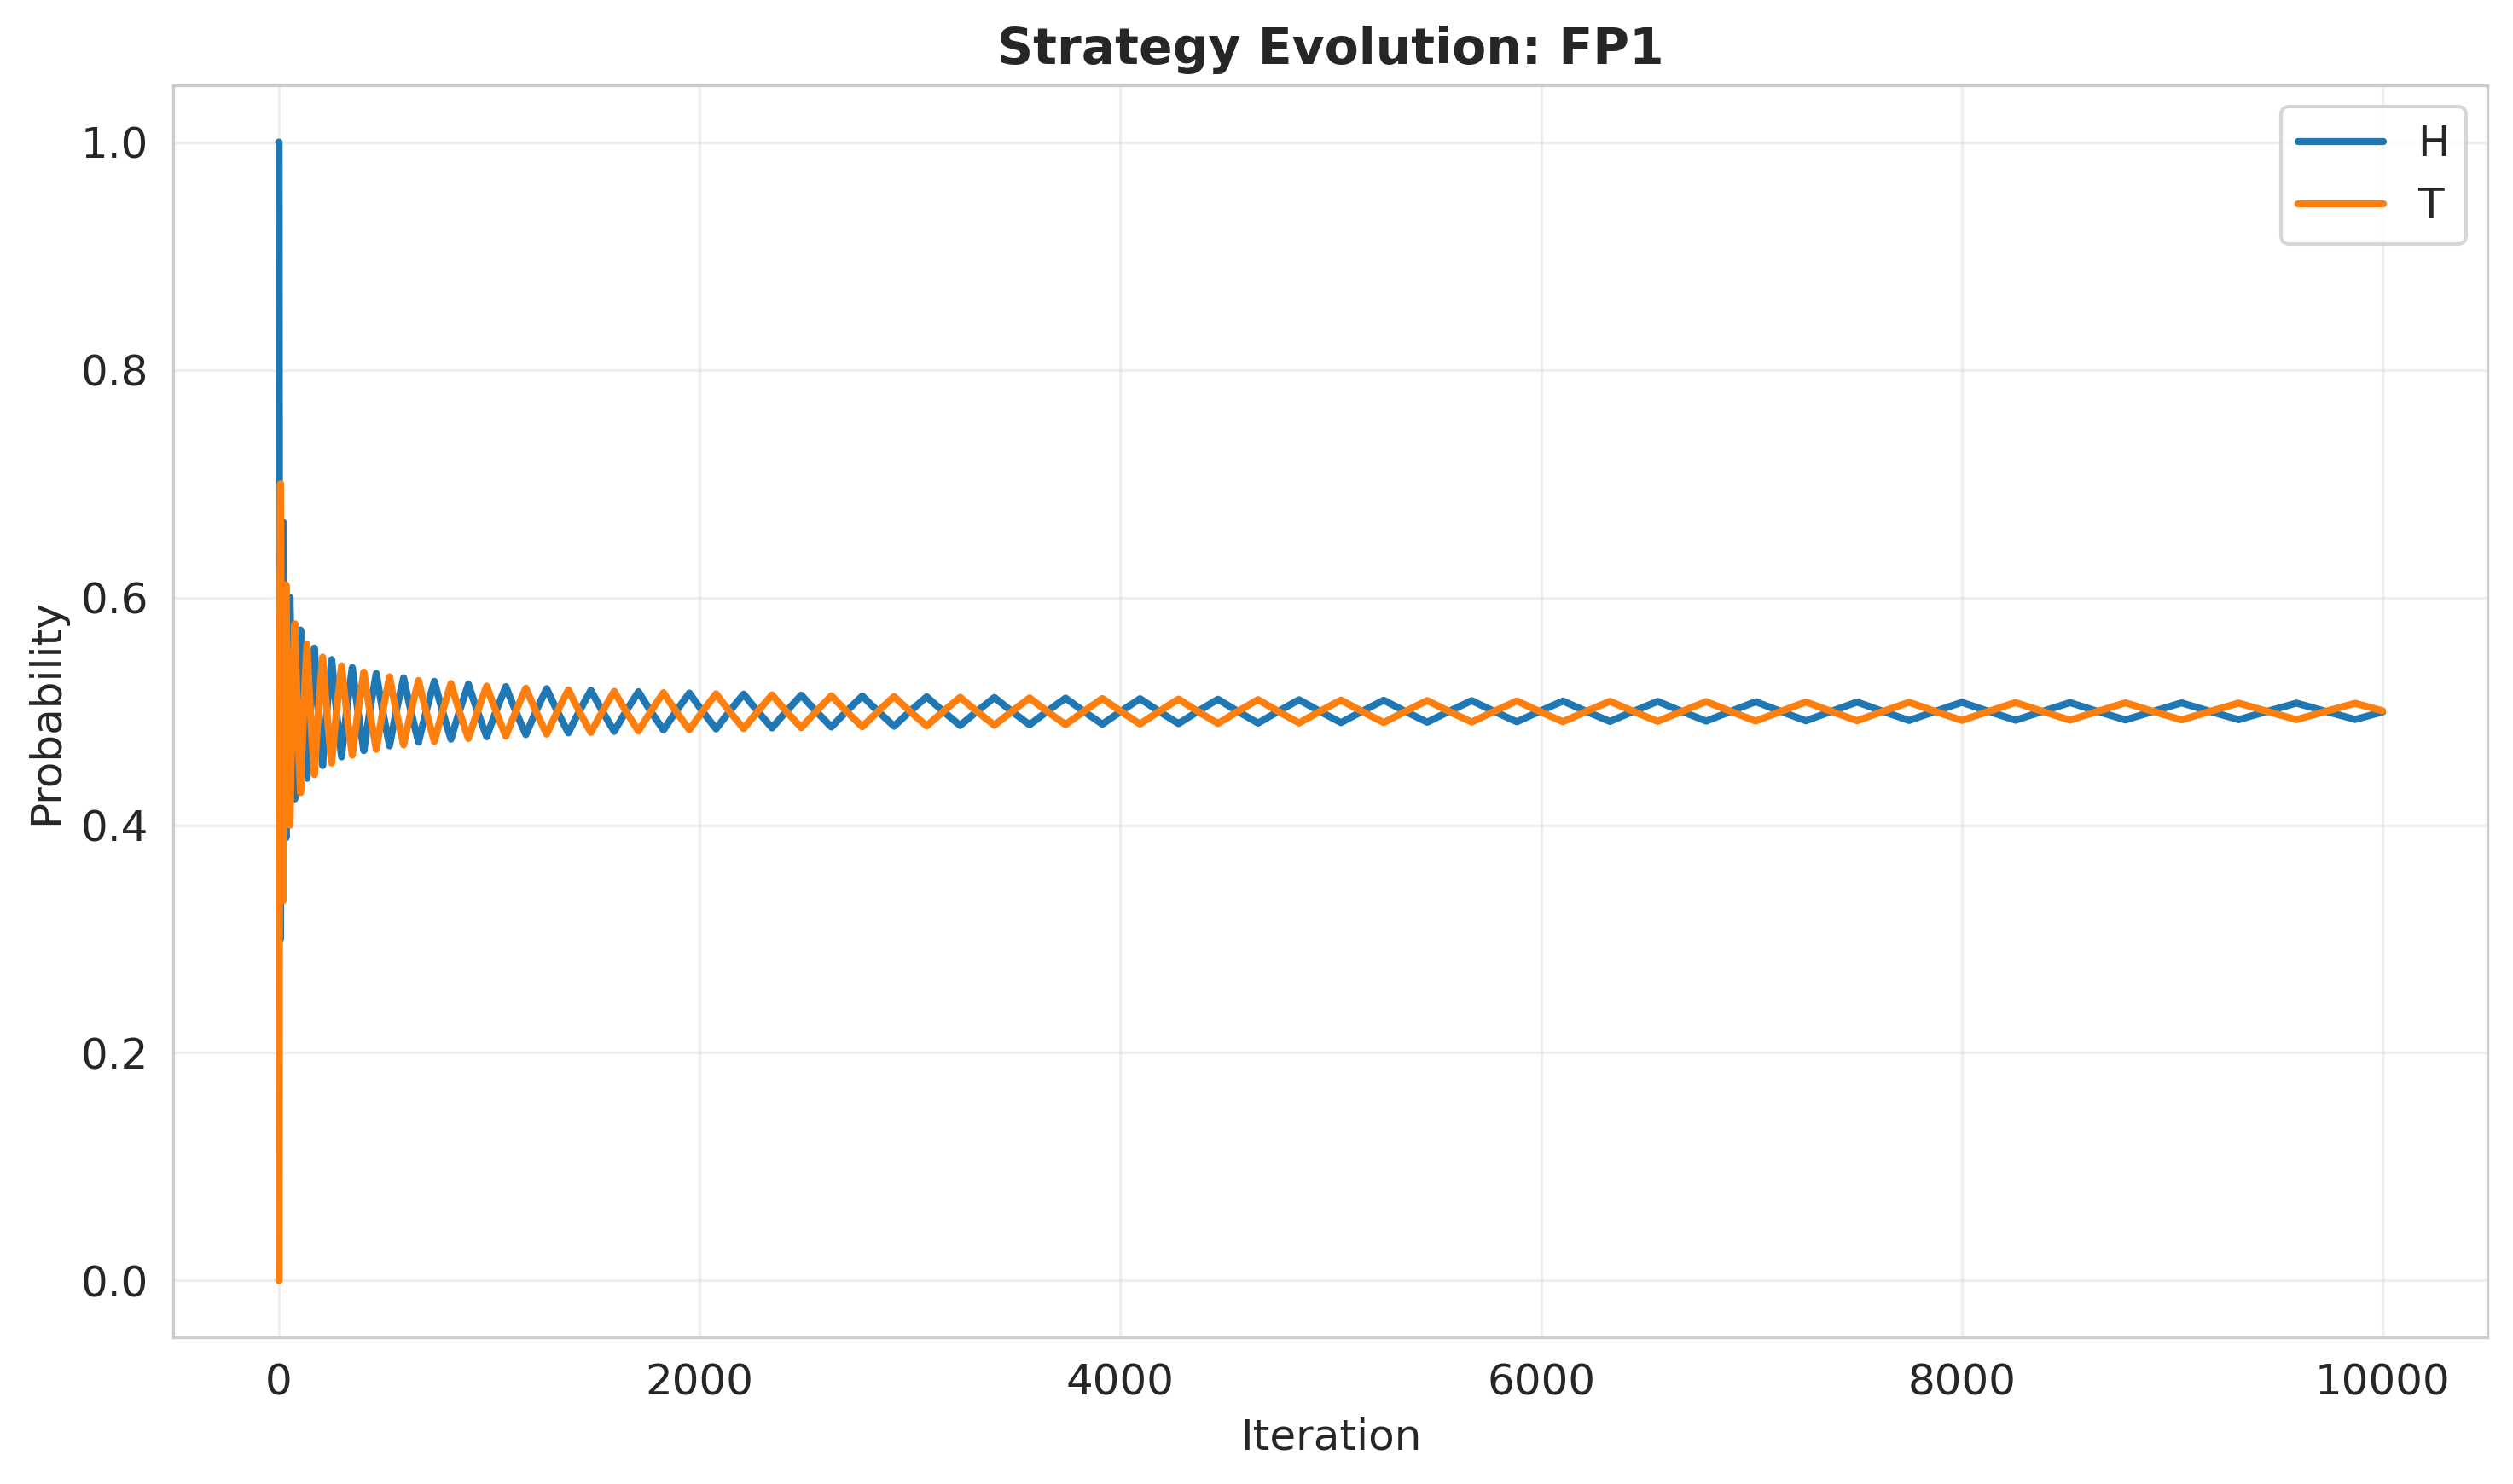
\includegraphics[width=0.8\textwidth]{../../results/plots/matching_pennies/FP vs FP/strategy1.png}
\caption{Εξέλιξη της πιθανότητας να παίξει «Heads» ο Παίκτης 1 (FP1). Η καμπύλη τείνει στο 0.5.}
\end{figure}

\begin{figure}[ht]
\centering
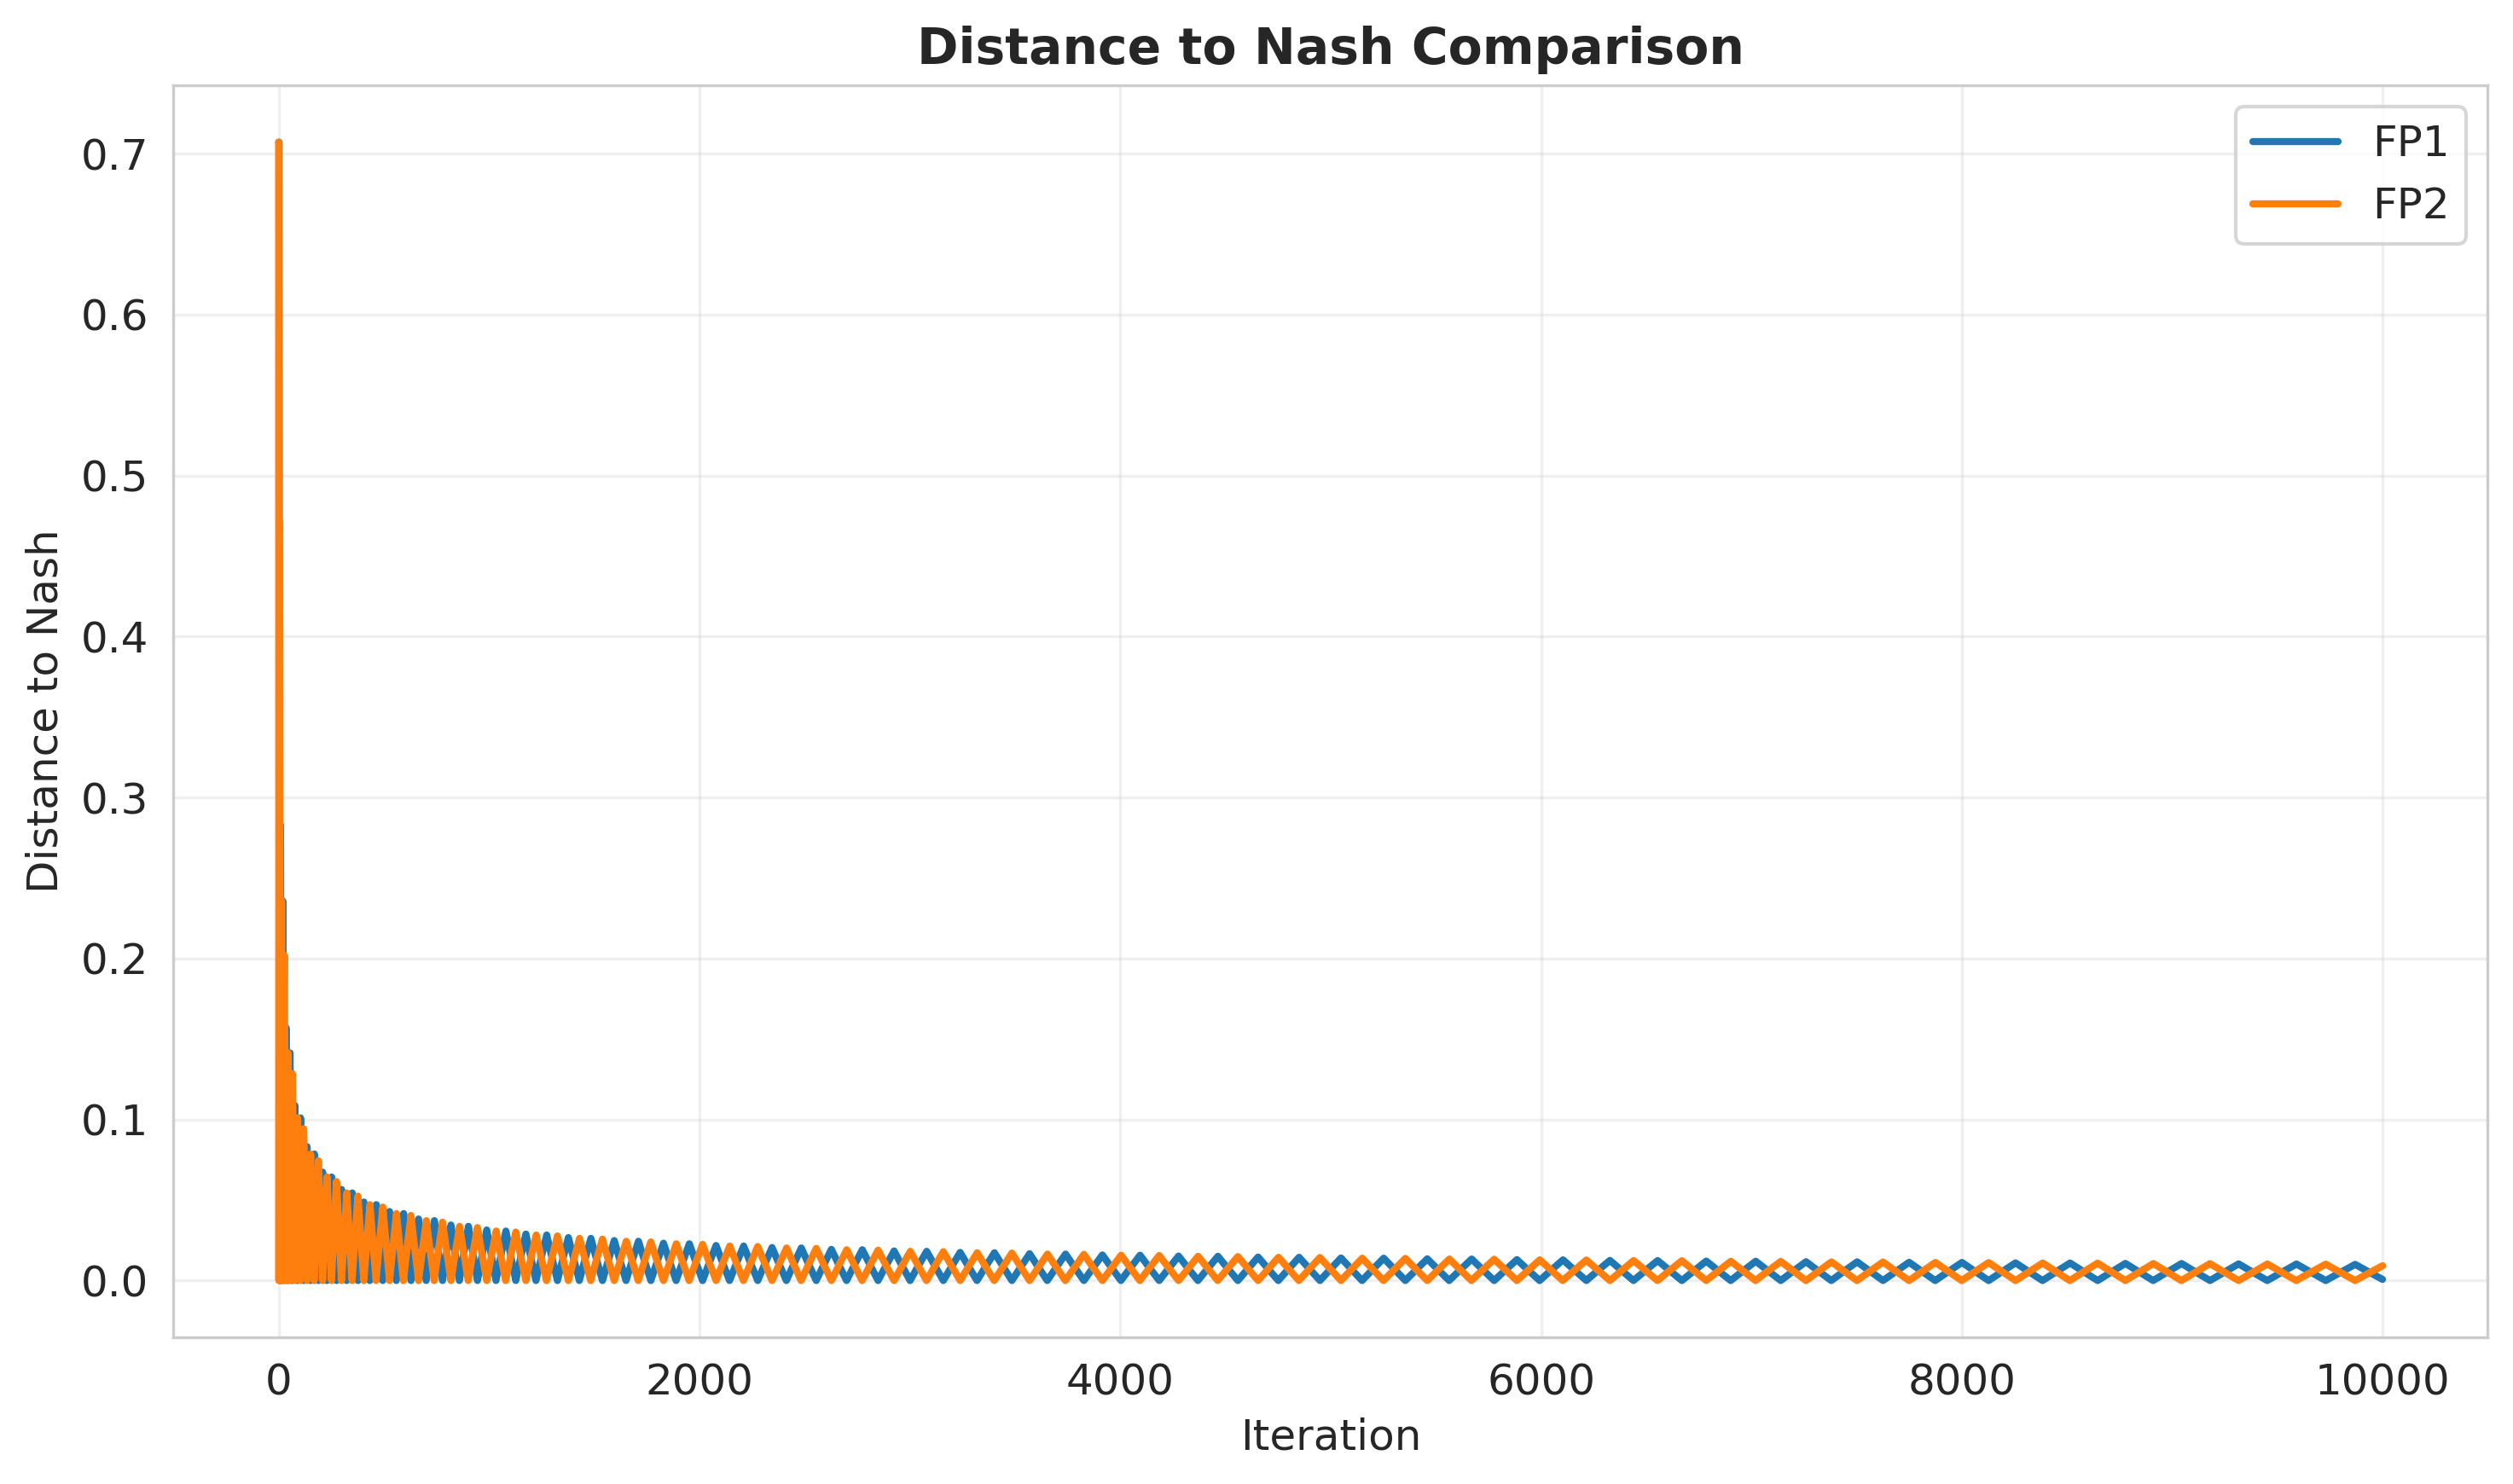
\includegraphics[width=0.8\textwidth]{../../results/plots/matching_pennies/FP vs FP/distance_comparison.png}
\caption{Ευκλείδεια απόσταση της εμπειρικής στρατηγικής από το Nash (0.5, 0.5). Και οι δύο πράκτορες έχουν απόσταση κοντά στο 0.}
\end{figure}

\begin{figure}[ht]
\centering
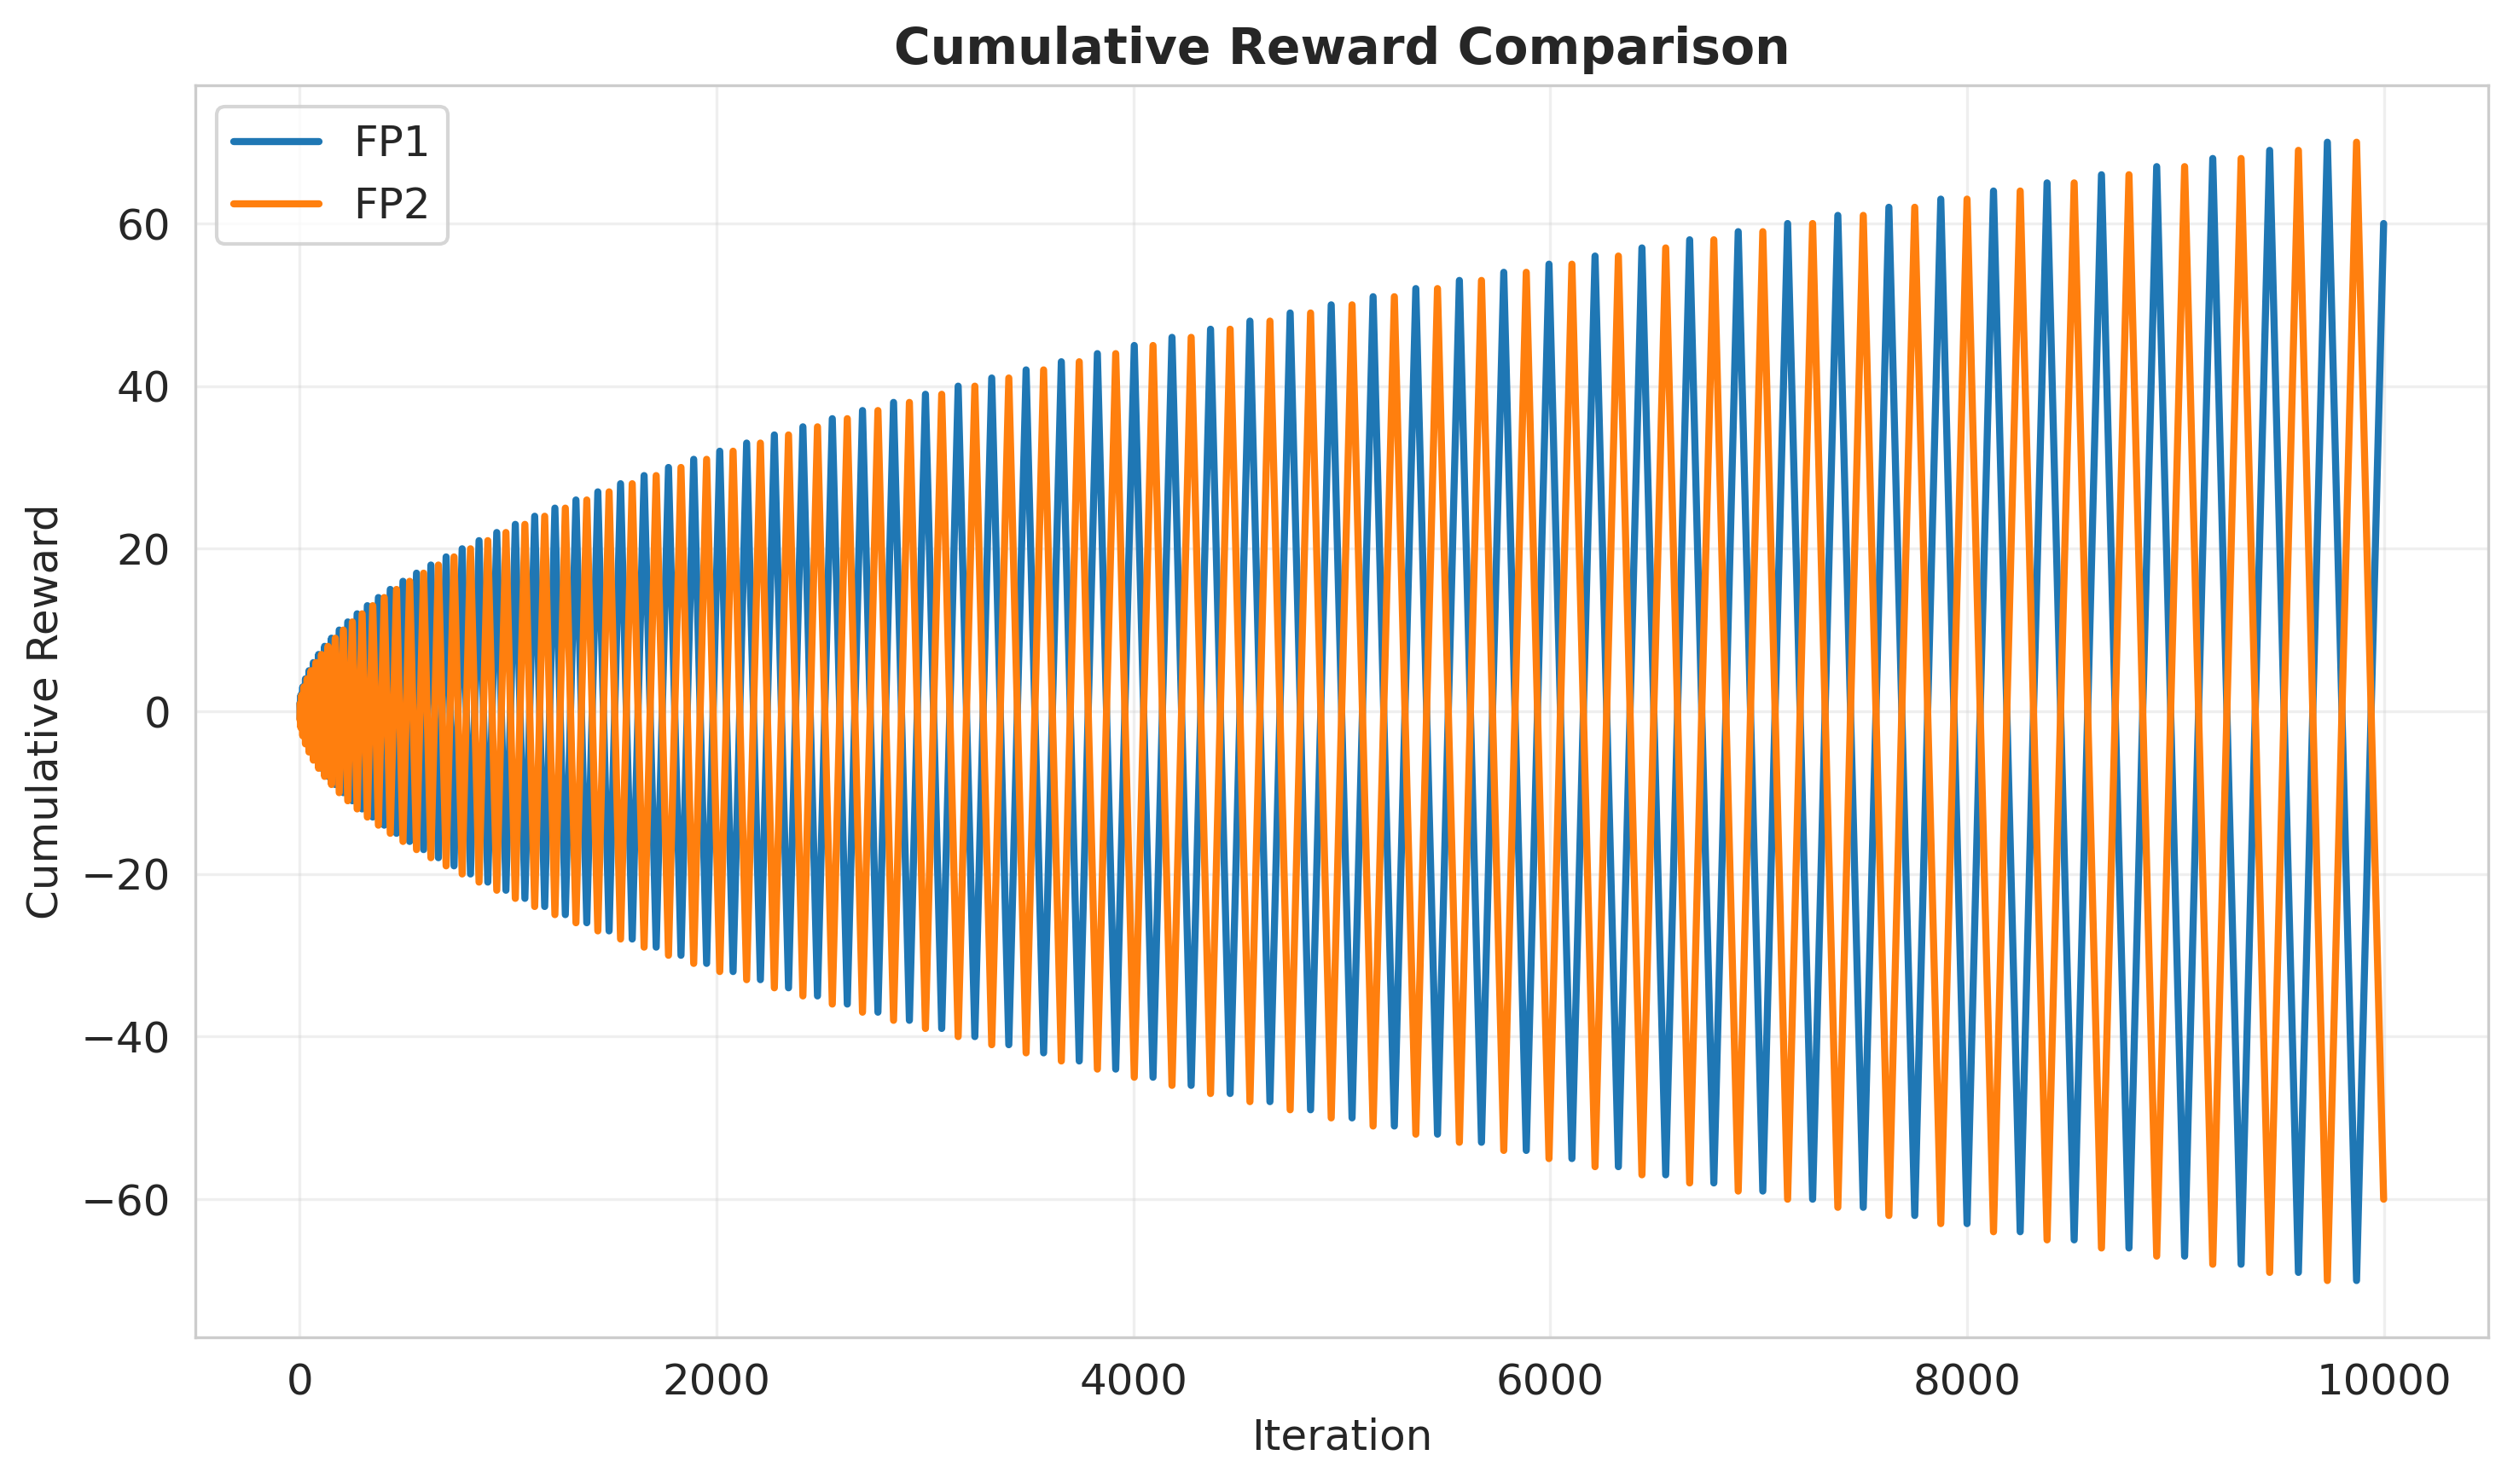
\includegraphics[width=0.8\textwidth]{../../results/plots/matching_pennies/FP vs FP/reward_comparison.png}
\caption{Cumulative reward. Οι καμπύλες παραμένουν κοντά στο μηδέν με μικρή τελική διαφορά (±60).}
\end{figure}

\subsubsection{Β. FP vs RL}

Εδώ ο Row Player είναι FP και ο Column Player είναι Q-learning (lr=0.1, \(\varepsilon\)=0.1). Στόχος: να δούμε αν το RL μπορεί να εκμεταλλευτεί την προβλεψιμότητα της FP.

Αποτελέσματα: FP distance 0.0000, RL 0.6642. FP cumulative −374, RL +374. Average −0.0374 / +0.0374. FP external regret 388, RL −374.

Η FP παραμένει στο Nash (απόσταση 0), αλλά ο RL δεν συγκλίνει στο NE· η απόστασή του παραμένει υψηλή (0.6642). Ο RL μαθαίνει να προβλέπει την determinist αντίδραση της FP (best response στο belief) και την εκμεταλλεύεται· γι' αυτό το cumulative reward του RL είναι +374 και της FP −374. Το external regret της FP αυξάνεται (388)· η FP δεν είναι no-regret απέναντι σε αυτόν τον δυναμικό αντίπαλο. Το αρνητικό regret του RL (−374) αντιστοιχεί στο ότι κέρδισε περισσότερο από το «best fixed action in hindsight» λόγω της προσαρμοστικής του συμπεριφοράς. Το βασικό σημείο είναι ότι «κοντά στο Nash» δεν συνεπάγεται «κερδίζω» όταν ο αντίπαλος δεν είναι στάσιμος. Ο RL, μέσω προσαρμογής, μπορεί να βρει patterns που αυξάνουν reward στο συγκεκριμένο horizon, ακόμη κι αν η συμπεριφορά του δεν μοιάζει καθόλου με Nash.

\begin{figure}[ht]
\centering
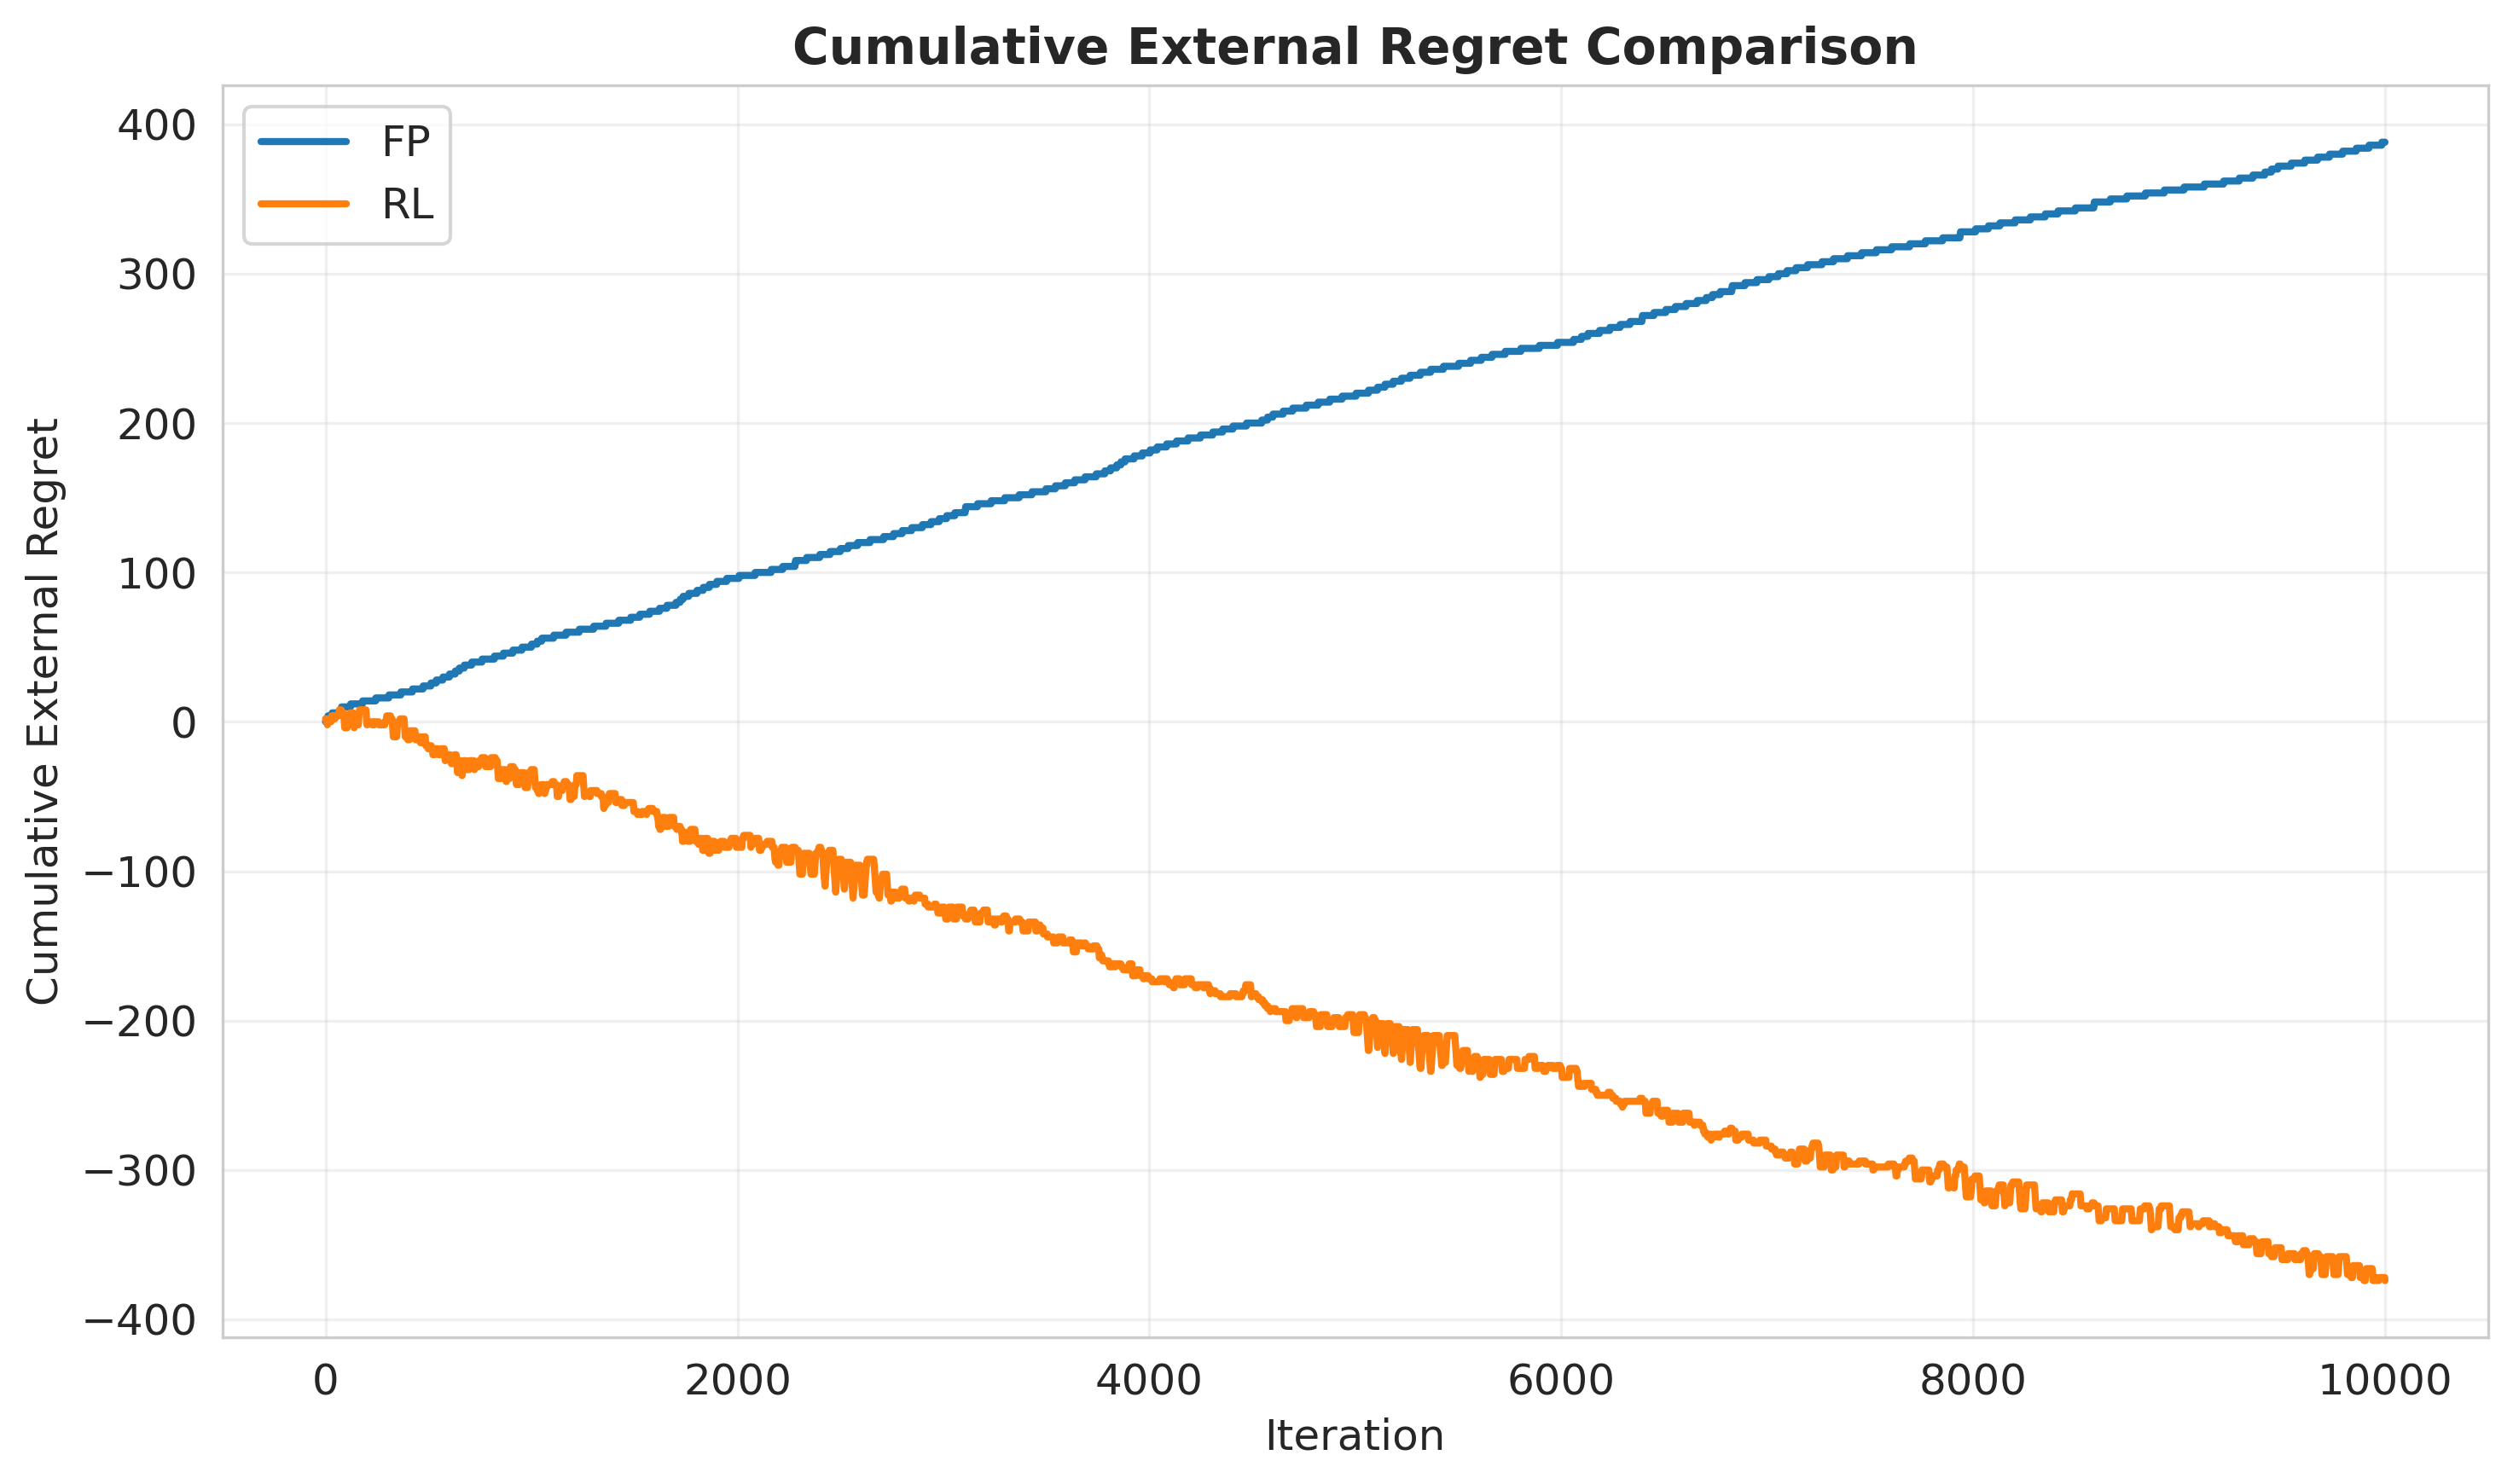
\includegraphics[width=0.8\textwidth]{../../results/plots/matching_pennies/FP vs RL/external_regret.png}
\caption{Συσσωρευμένο external regret. Η FP (θετική καμπύλη) έχει γραμμικά αυξανόμενο regret· ο RL (αρνητική) έχει sublinear/αρνητικό regret.}
\end{figure}

\begin{figure}[ht]
\centering
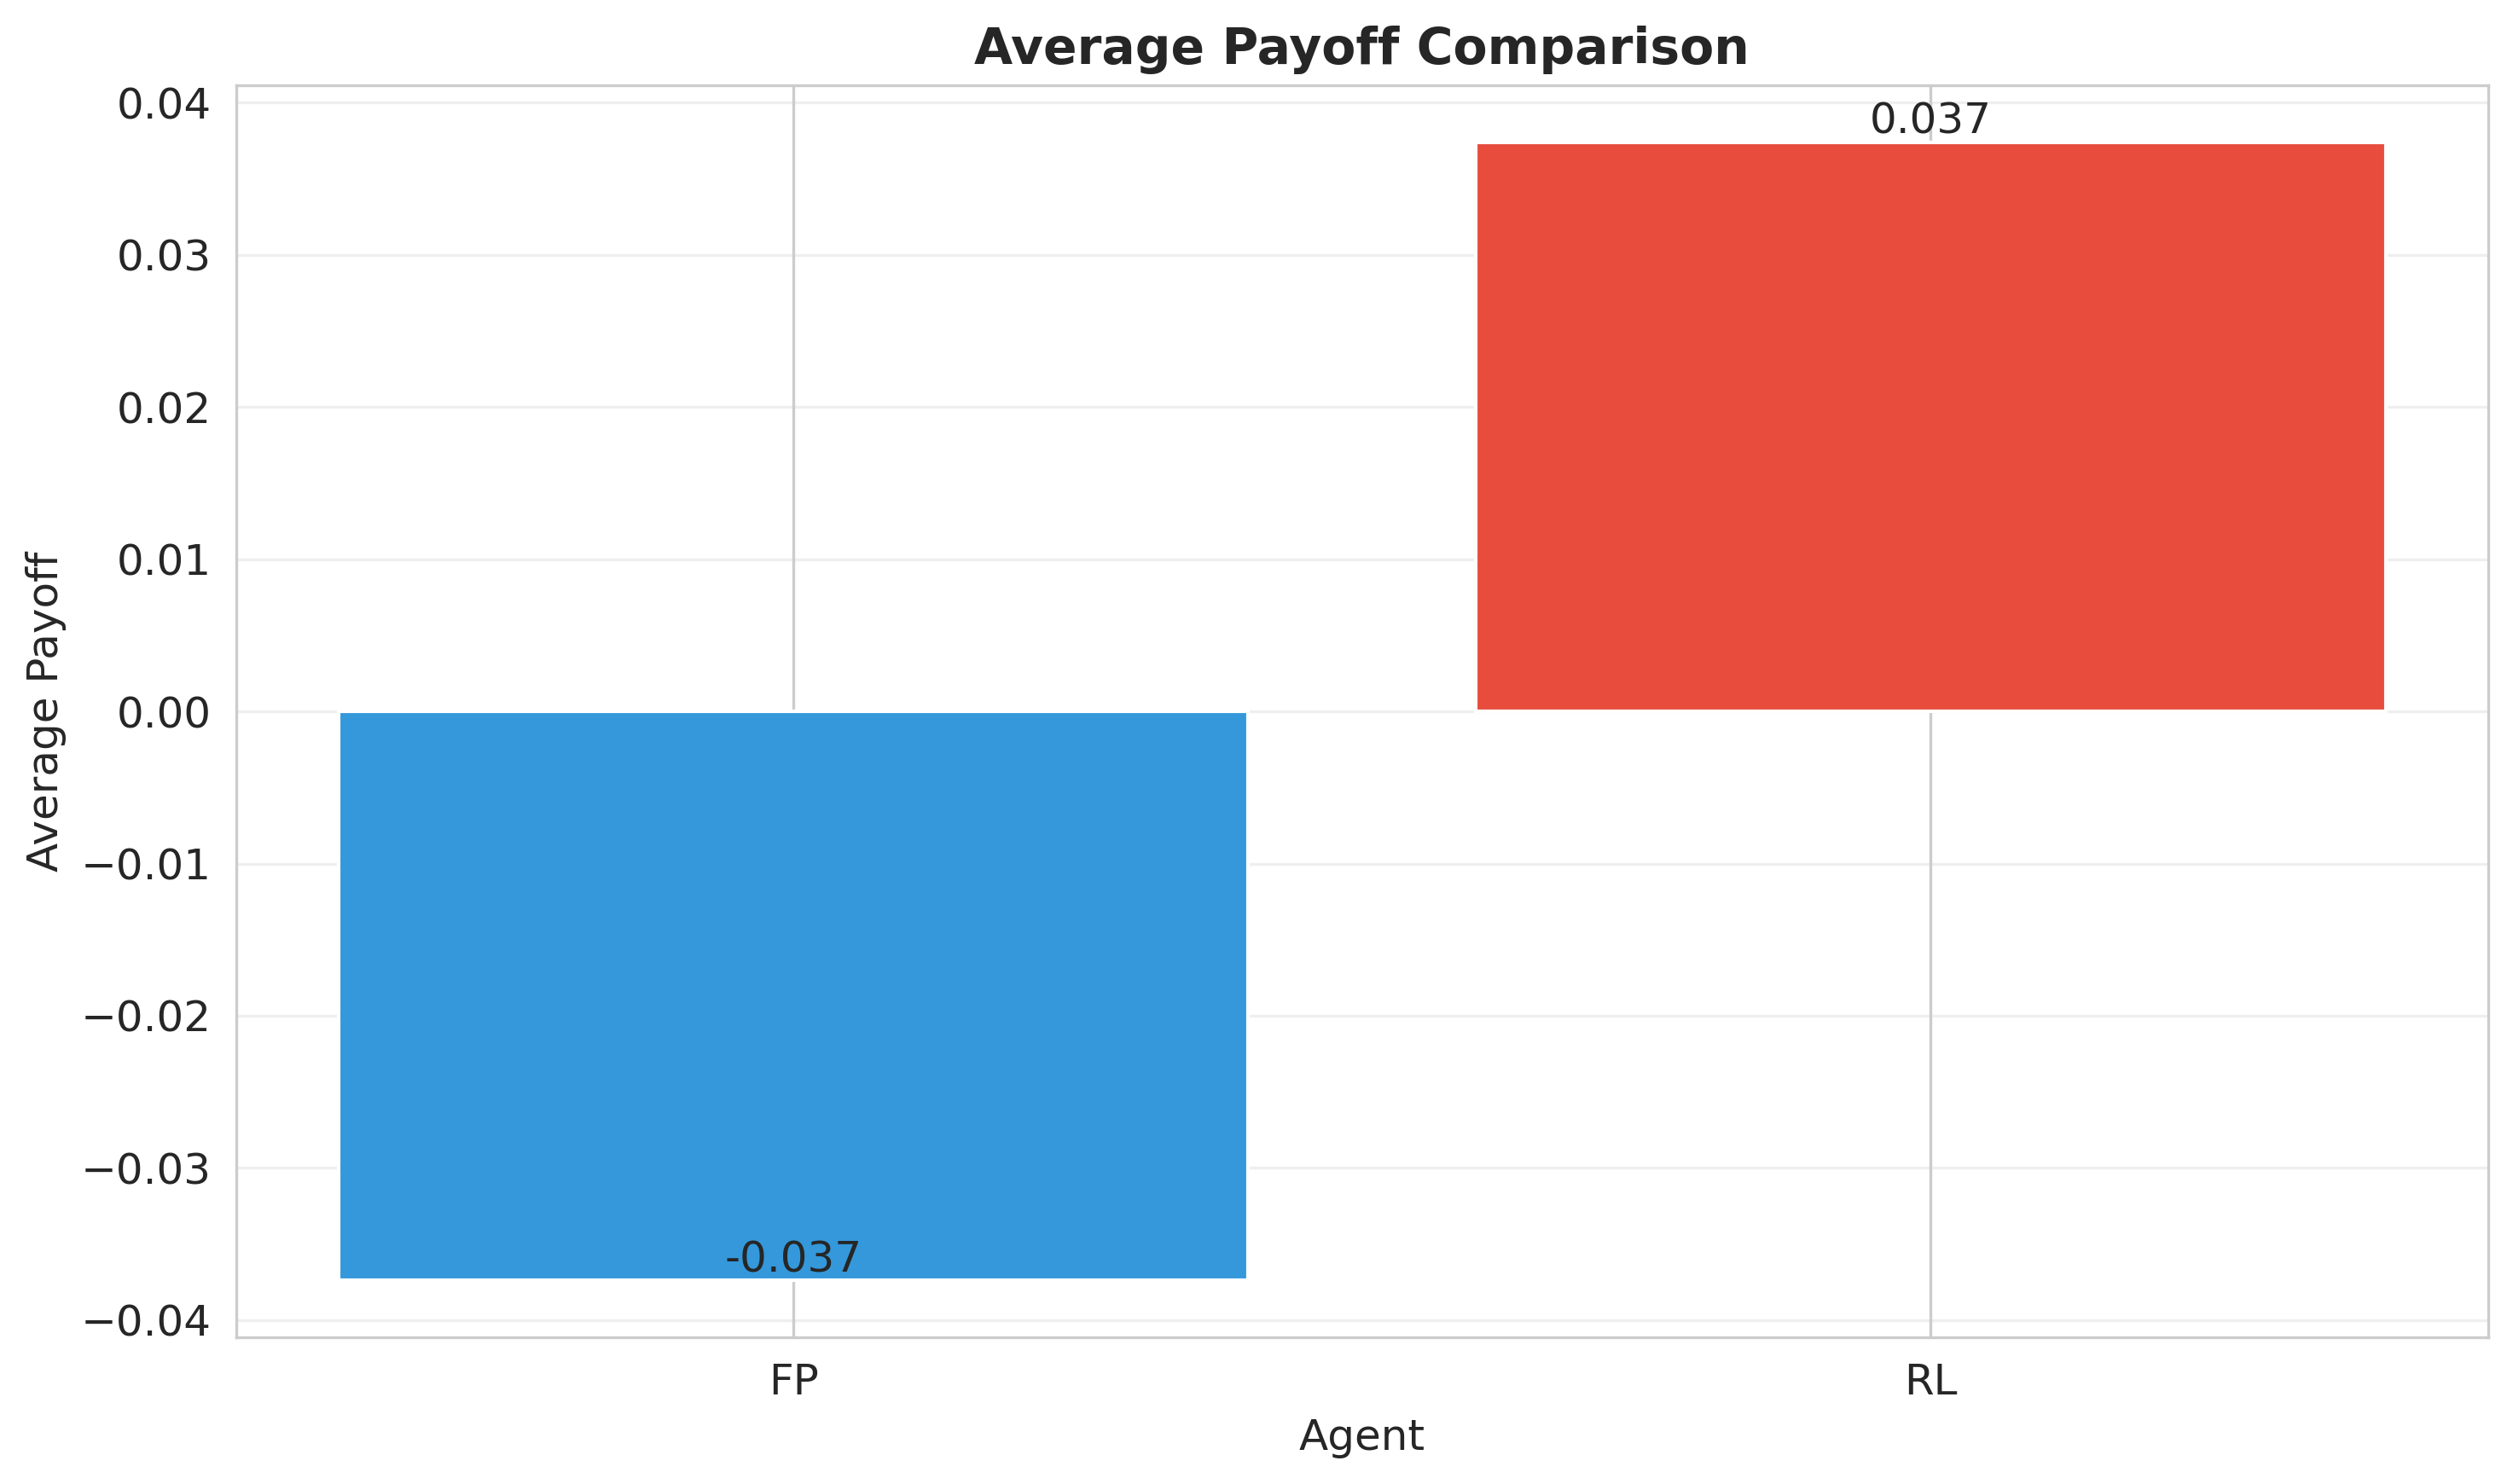
\includegraphics[width=0.8\textwidth]{../../results/plots/matching_pennies/FP vs RL/avg_payoff.png}
\caption{Μέσο payoff ανά γύρο. Ο RL έχει θετικό μέσο payoff, η FP αρνητικό.}
\end{figure}

\begin{figure}[ht]
\centering
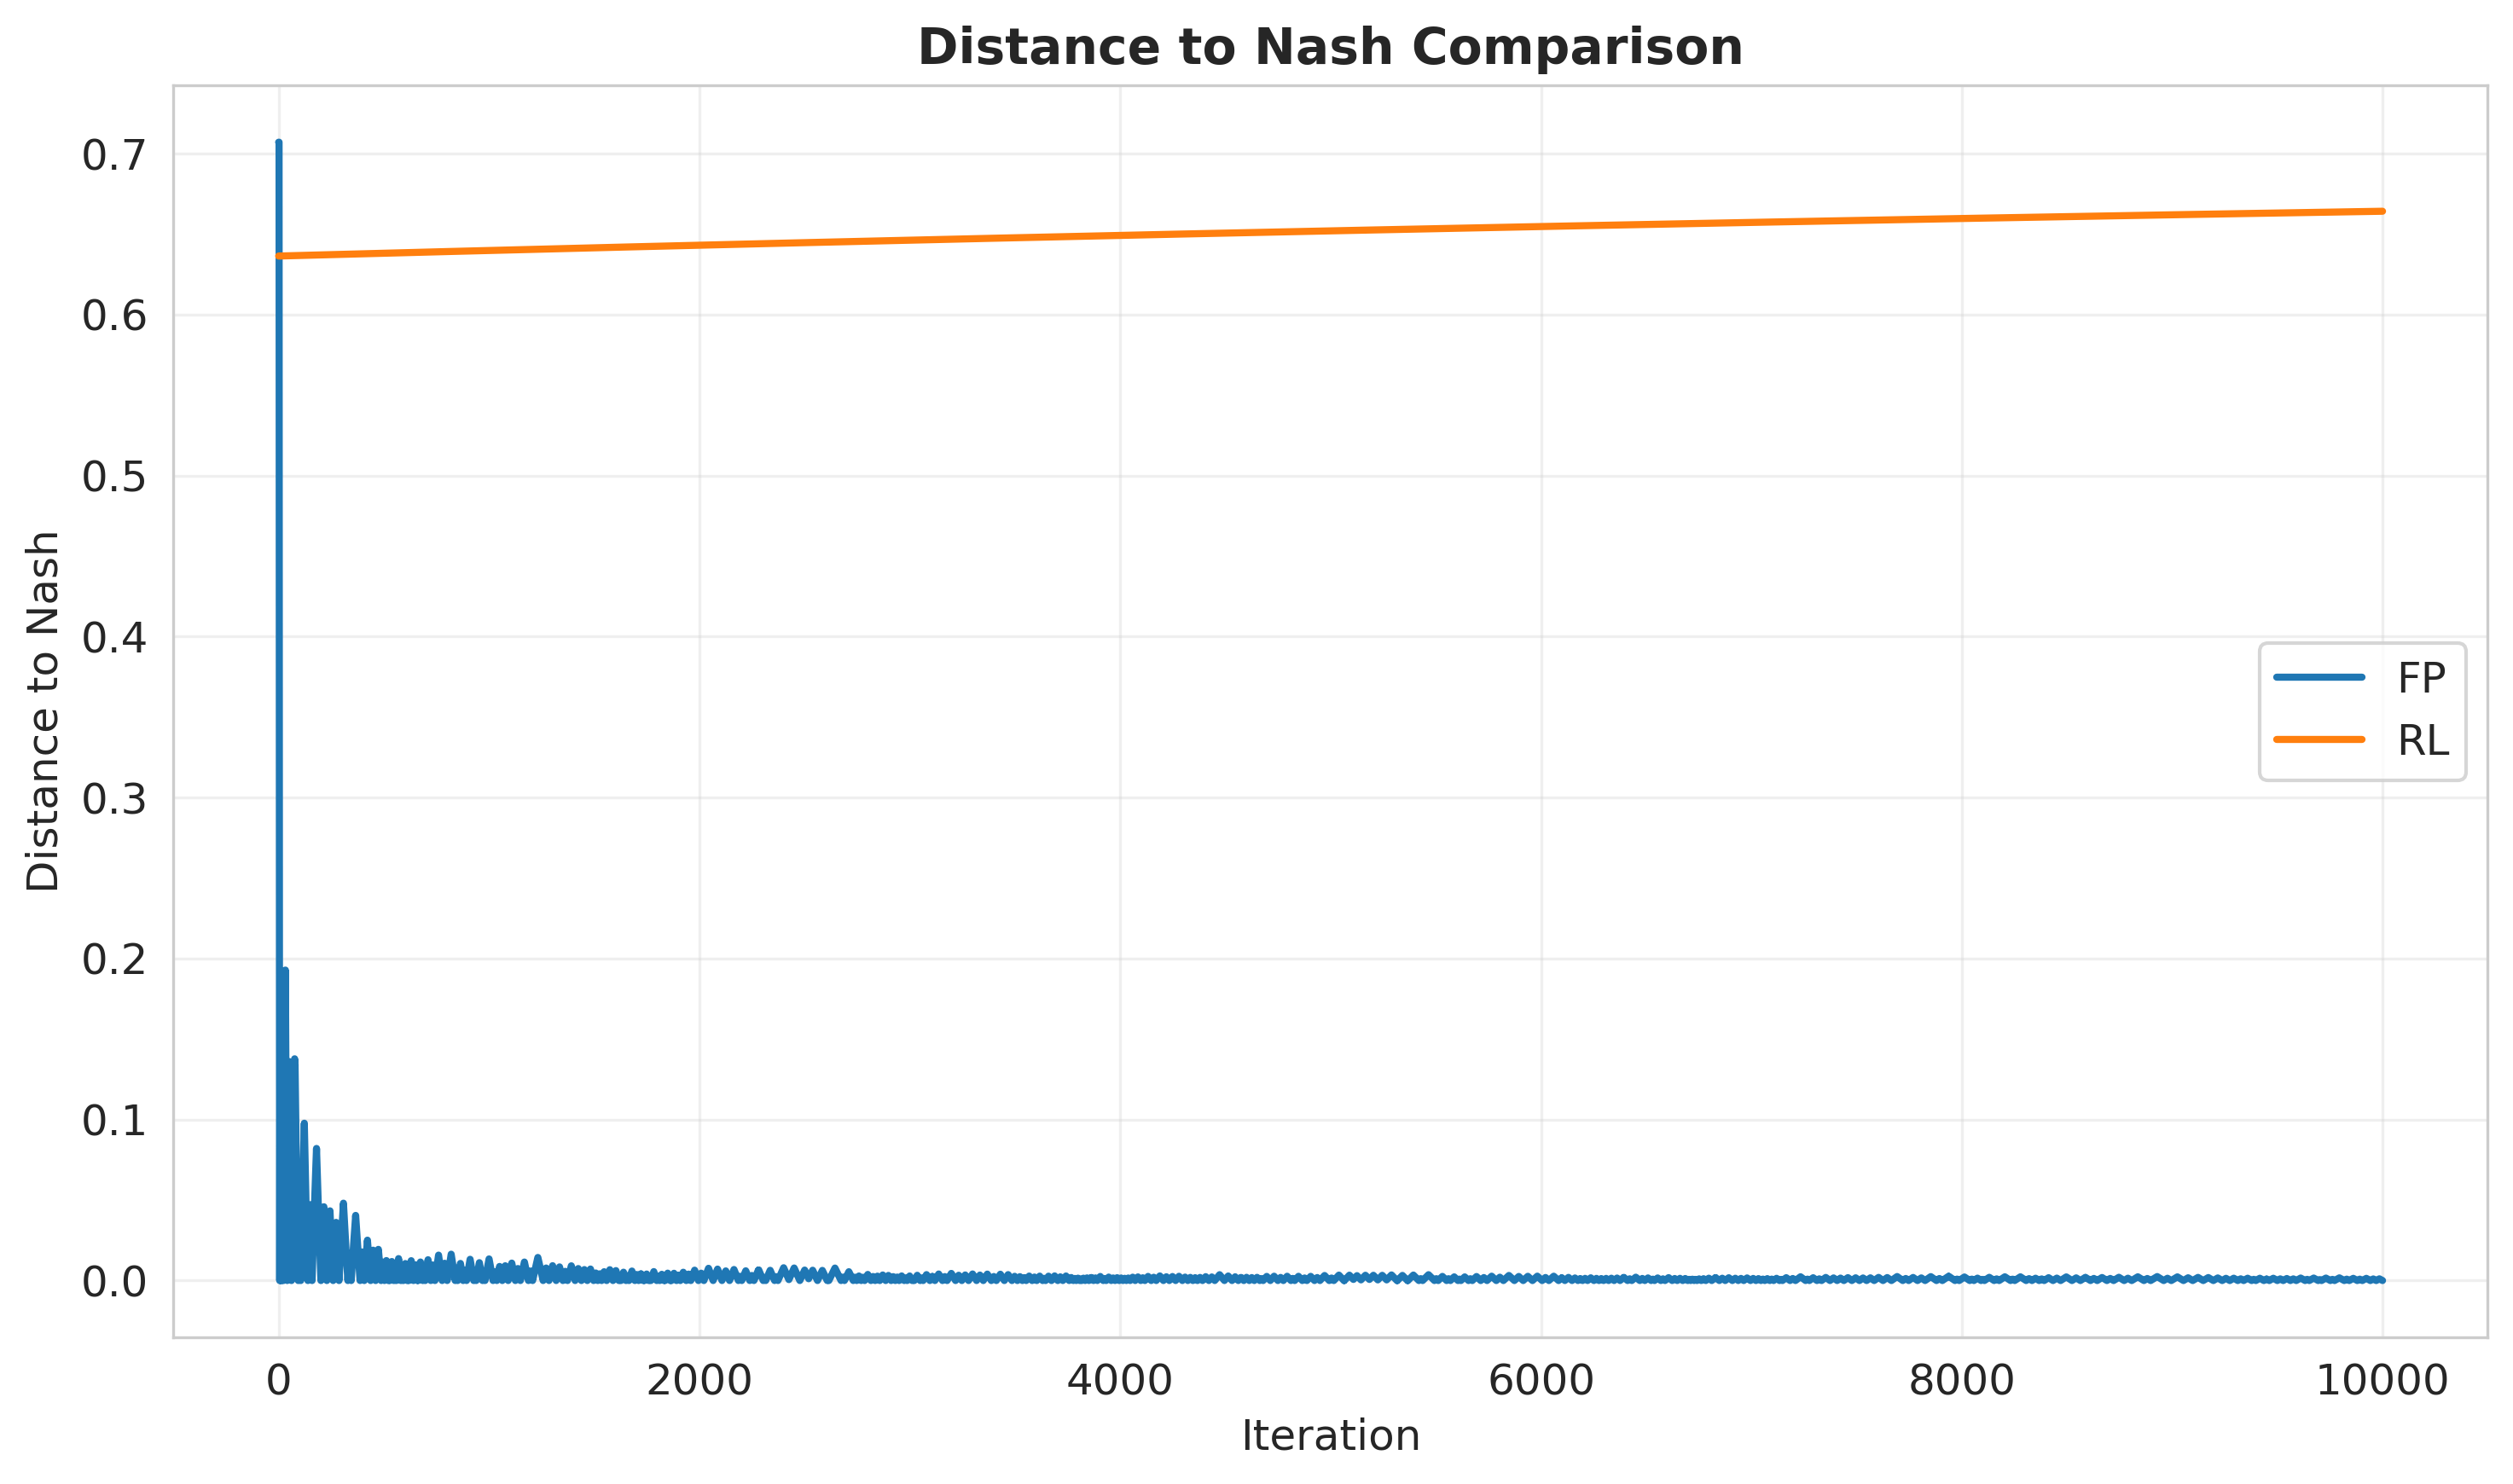
\includegraphics[width=0.8\textwidth]{../../results/plots/matching_pennies/FP vs RL/distance_comparison.png}
\caption{Απόσταση από Nash. FP πλησιάζει 0, RL παραμένει περίπου 0.66.}
\end{figure}

\begin{figure}[ht]
\centering
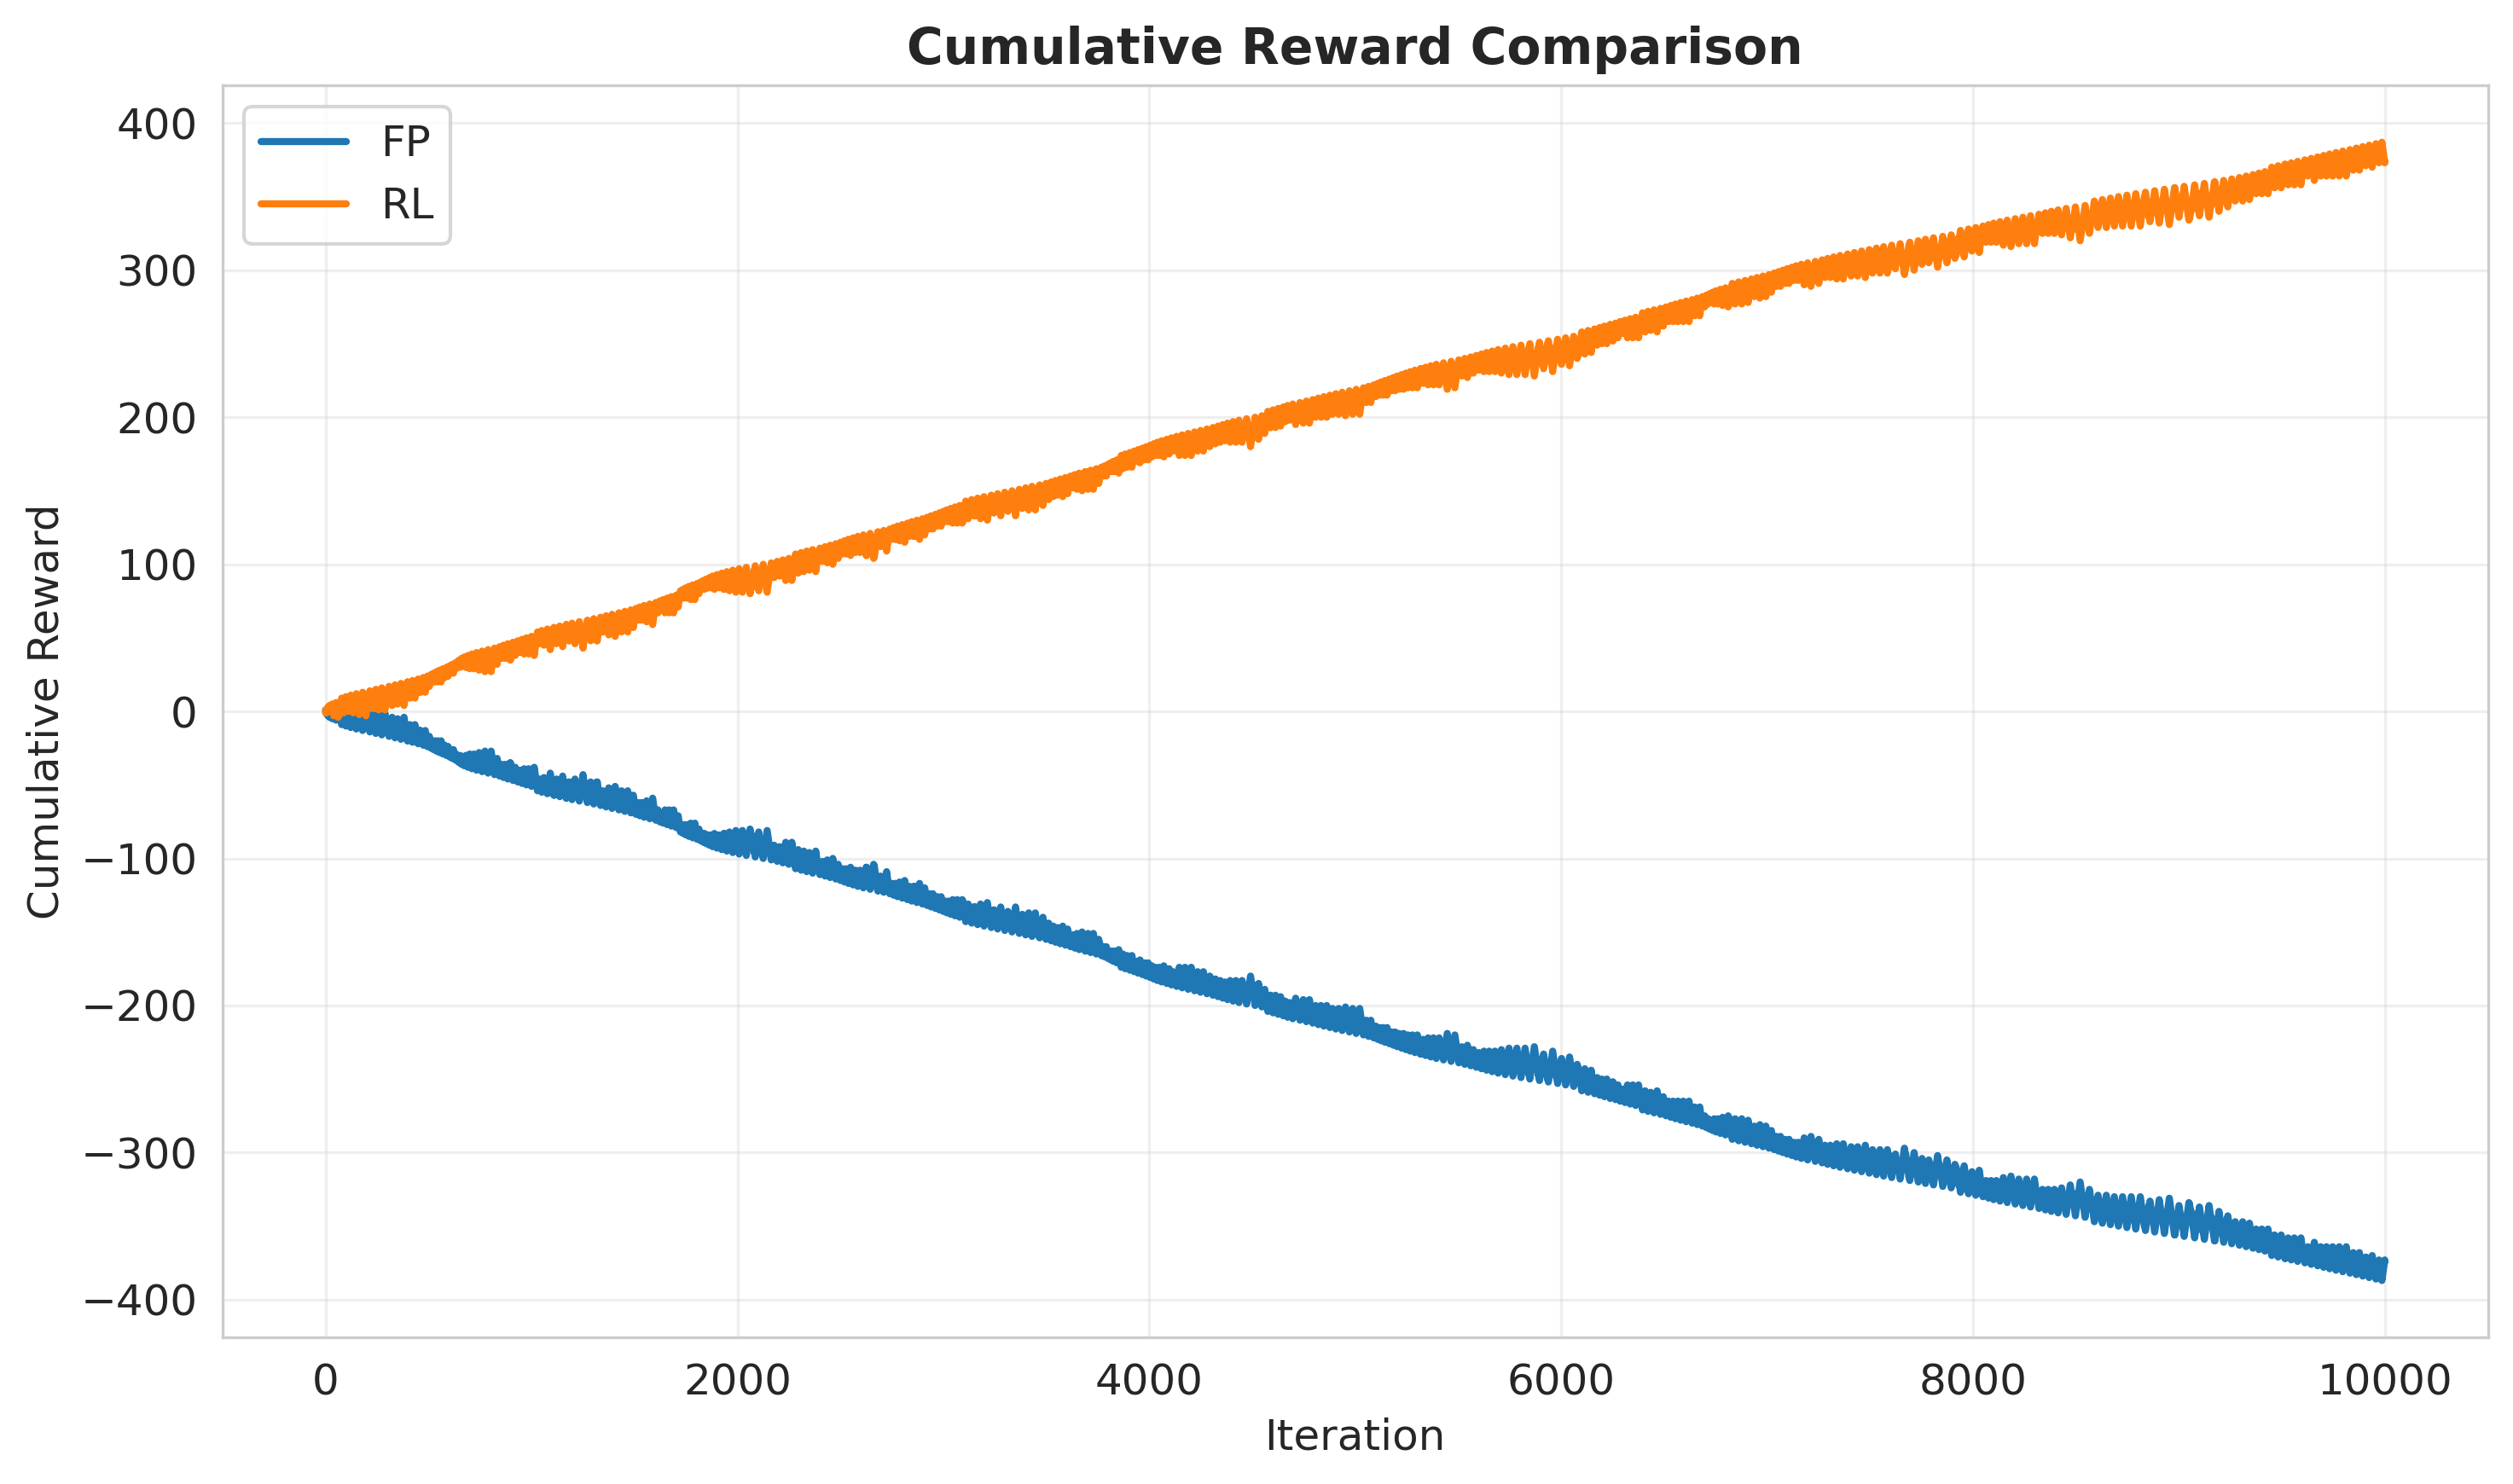
\includegraphics[width=0.8\textwidth]{../../results/plots/matching_pennies/FP vs RL/reward_comparison.png}
\caption{Cumulative reward. RL +374, FP −374.}
\end{figure}

Συμπέρασμα για FP vs RL (Matching Pennies): Η FP είναι βέλτιστη για εύρεση Nash σε στατικό ή συμμετρικό περιβάλλον, αλλά ευάλωτη σε αντιπάλους που μαθαίνουν τα patterns της· ο RL εκμεταλλεύεται αυτή την προβλεψιμότητα και πετυχαίνει υψηλό cumulative reward εις βάρος της ισορροπίας.

\subsubsection{Γ. RL vs RL}

Αποτελέσματα: RL1 και RL2 distance 0.6642. RL1 cumulative −4, RL2 +4. Average ±0.0004.

Καμία πλευρά δεν συγκλίνει στο Nash (απόσταση ~0.66). Τα cumulative rewards είναι σχεδόν μηδέν (±4 σε 10.000 γύρων) — δεν υπάρχει συστηματική εκμετάλλευση. Το περιβάλλον είναι non-stationary (ο αντίπαλος αλλάζει συνεχώς) και οι υποθέσεις σύγκλισης του Q-learning δεν ικανοποιούνται. Η διαφορά με το FP vs RL είναι αισθητή: εδώ κανένας δεν «κρατάει» σταθερή στρατηγική αρκετά για να εκμεταλλευτεί ο άλλος.

Εκτελέσαμε επίσης hyperparameter sweep (5.000 iterations ανά ζεύγος) για να μελετήσουμε την exploitability της τελικής στρατηγικής του RL1 ως συνάρτηση του learning rate (\(\alpha\)) και του epsilon (\(\varepsilon\)). Η exploitability μετρά πόσο μπορεί να κερδίσει ο αντίπαλος παίζοντας best response απέναντι στη στρατηγική μας — μηδέν στο Nash, μέγιστο 2 στο Matching Pennies για καθαρή στρατηγική.

\begin{center}
\small
\begin{tabular}{@{}lccc@{}}
\toprule
 & \(\varepsilon=0.05\) & \(\varepsilon=0.10\) & \(\varepsilon=0.20\) \\
\midrule
\(\alpha=0.01\) & 1.9099 & 1.8217 & 1.6508 \\
\(\alpha=0.10\) & 1.9099 & 1.8217 & 1.6508 \\
\(\alpha=0.50\) & 1.9099 & 1.8217 & 1.6508 \\
\bottomrule
\end{tabular}
\end{center}

Οι τιμές (1.65--1.91) είναι υψηλές και συνεπείς με το ότι το RL δεν συγκλίνει στο NE. Παρατηρούμε ότι η exploitability εξαρτάται \emph{μόνο από το \(\varepsilon\)}, όχι από το \(\alpha\). Μεγαλύτερο \(\varepsilon\) → πιο ομοιόμορφη προσέγγιση της στρατηγικής μέσω \eng{get\_strategy()} → πιο κοντά στο (0.5, 0.5) → μικρότερη exploitability. Το learning rate δεν επηρεάζει την τελική exploitability γιατί μετά από 5.000 γύρους τα Q-values και τα argmax έχουν σταθεροποιηθεί παρόμοια ανεξάρτητα από το \(\alpha\).

\begin{figure}[ht]
\centering
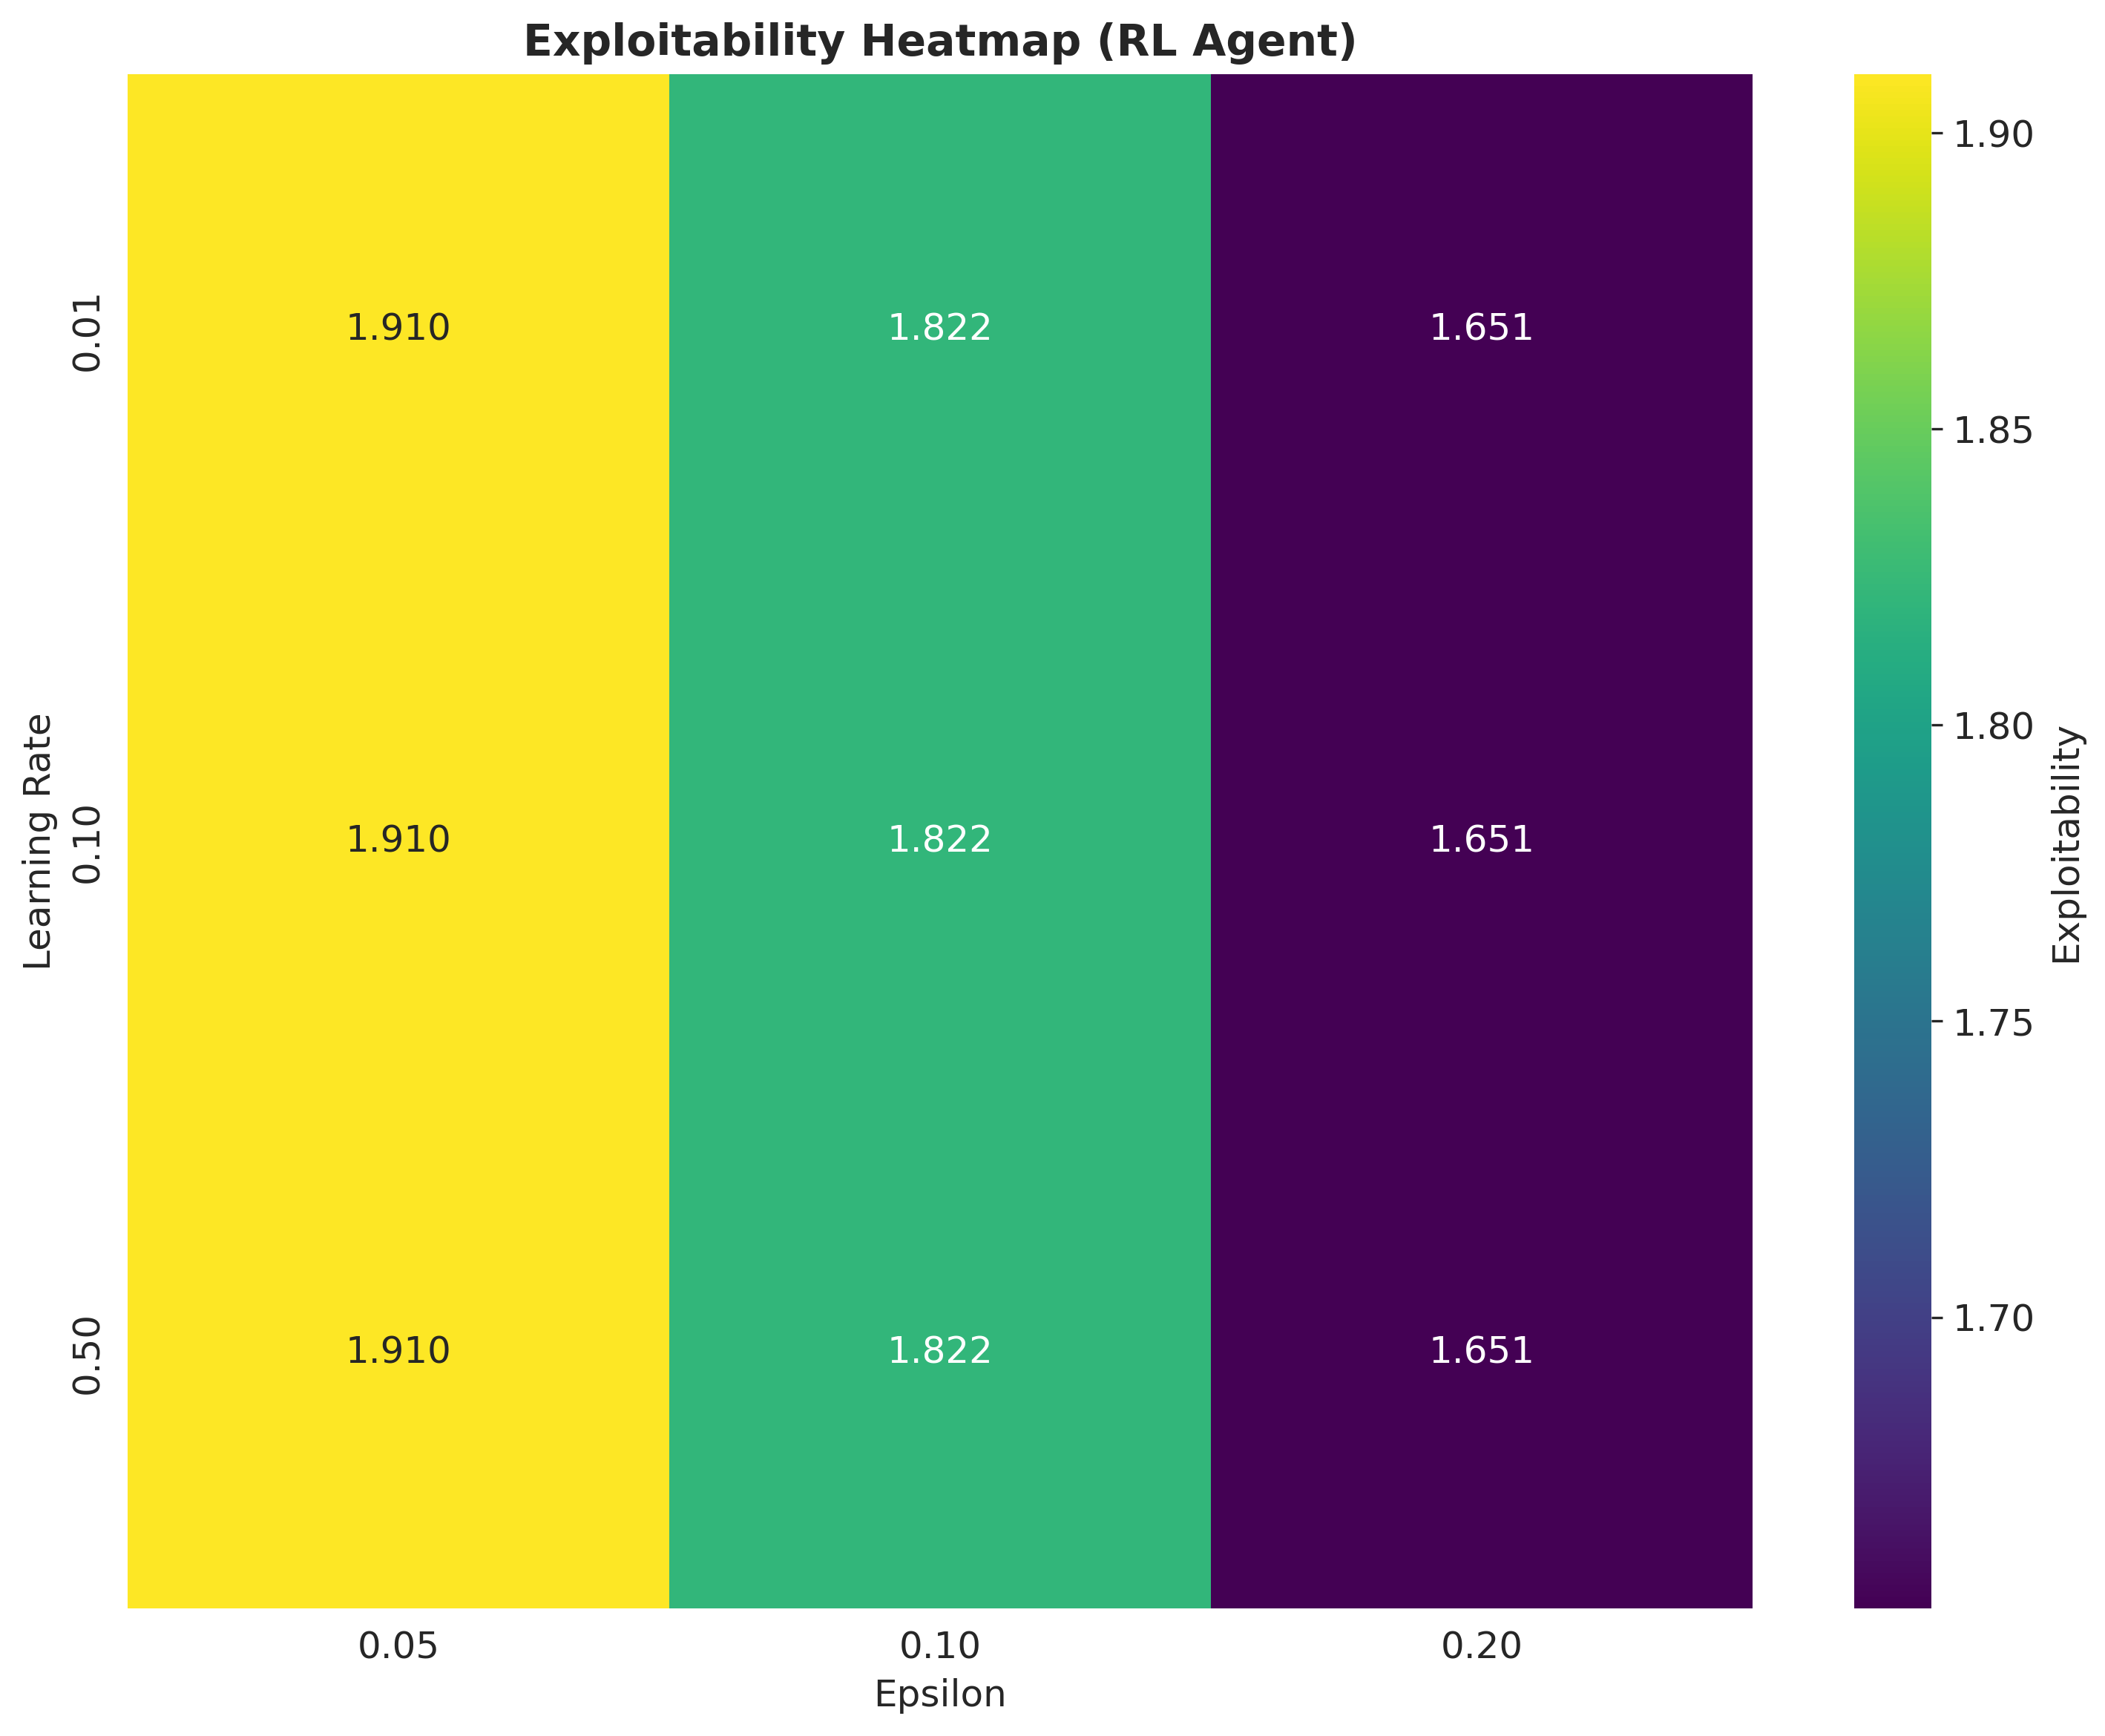
\includegraphics[width=0.8\textwidth]{../../results/plots/matching_pennies/RL vs RL/exploitability_heatmap.png}
\caption{Exploitability heatmap στο Matching Pennies (RL vs RL). Αξόνες: learning rate, epsilon. Υψηλές τιμές = οι learned στρατηγικές απέχουν από το Nash.}
\end{figure}

\subsection{Rock-Paper-Scissors (3×3)}

Το θεωρητικό NE είναι (1/3, 1/3, 1/3). Πειράματα: 10.000 iterations. Πηγές: \eng{results/plots/rock\_paper\_scissors/*/results.txt}.

\subsubsection{FP vs FP}

Αποτελέσματα: FP1 και FP2 distance 0.0032. Cumulative 0 / 0. Average 0.0000.

Τέλεια σύγκλιση: και οι δύο πράκτορες φτάνουν κοντά στο (1/3, 1/3, 1/3). Τα rewards είναι ακριβώς μηδενικά — συνεπή με το zero-sum στο NE, όπου το αναμενόμενο payoff και των δύο είναι 0. Η απόσταση 0.0032 είναι αμελητέα. Αυτό είναι η πιο «καθαρή» ένδειξη ισορροπιακής συμπεριφοράς: οι εμπειρικές στρατηγικές προσεγγίζουν το (1/3, 1/3, 1/3) και, λόγω συμμετρίας, δεν εμφανίζεται καθαρό πλεονέκτημα σε reward.

\subsubsection{FP vs RL}

Αποτελέσματα: FP distance 0.0152, RL 0.7670. FP cumulative −213, RL +213. Average −0.0213 / +0.0213. FP regret 234, RL −3.

Η FP πλησιάζει το Nash· ο RL παραμένει μακριά (0.7670). Ο RL κερδίζει +213 και έχει σχεδόν μηδενικό external regret (−3)· η FP έχει θετικό και αυξανόμενο regret (234). Η ερμηνεία ταυτίζεται με το Matching Pennies: ο RL παίζει best response στις μικρές στατιστικές αποκλίσεις της FP. Στο RPS οι αποκλίσεις είναι πιο «εκμεταλλεύσιμες» λόγω των τριών ενεργειών, οπότε ο RL πετυχαίνει καλή απόδοση. Το pattern επαναλαμβάνεται: το RL δεν συγκλίνει σε Nash, όμως εκμεταλλεύεται τη δυναμική του FP.

\begin{figure}[ht]
\centering
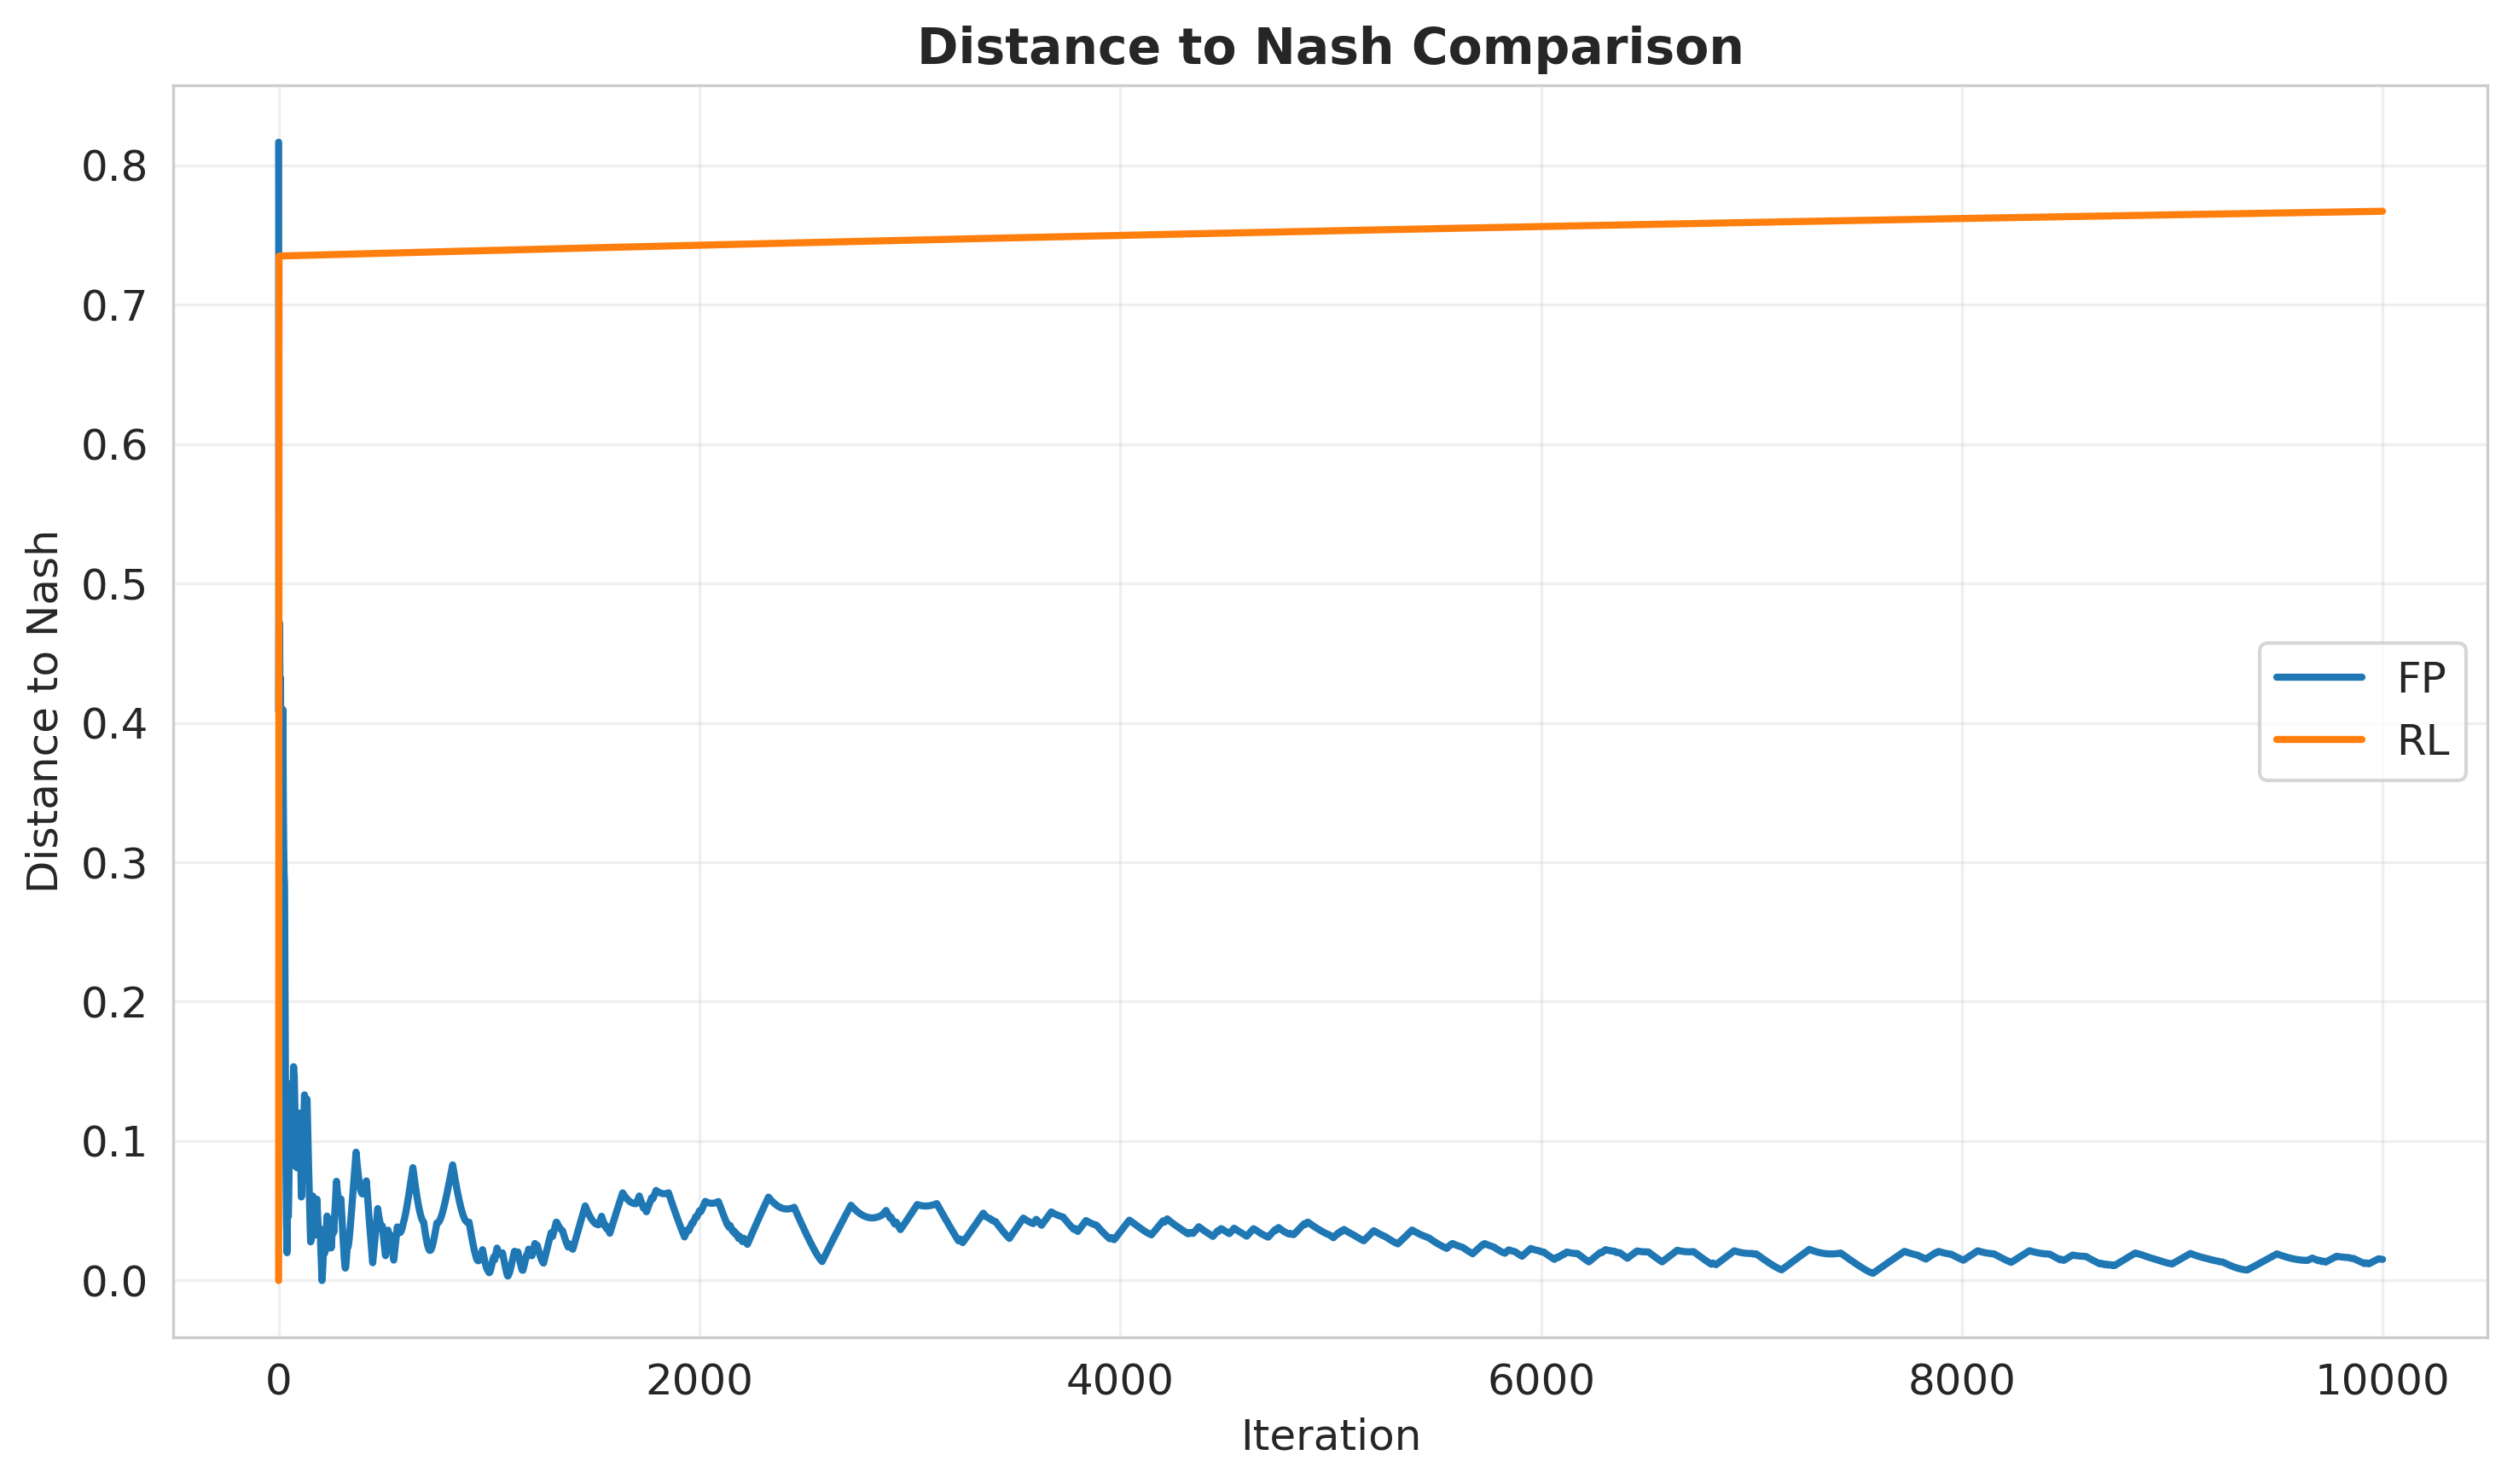
\includegraphics[width=0.8\textwidth]{../../results/plots/rock_paper_scissors/FP vs RL/distance_comparison.png}
\caption{Απόσταση από Nash στο RPS. FP (μπλε) κοντά στο 0, RL (πορτοκαλί) ~0.77.}
\end{figure}

\begin{figure}[ht]
\centering
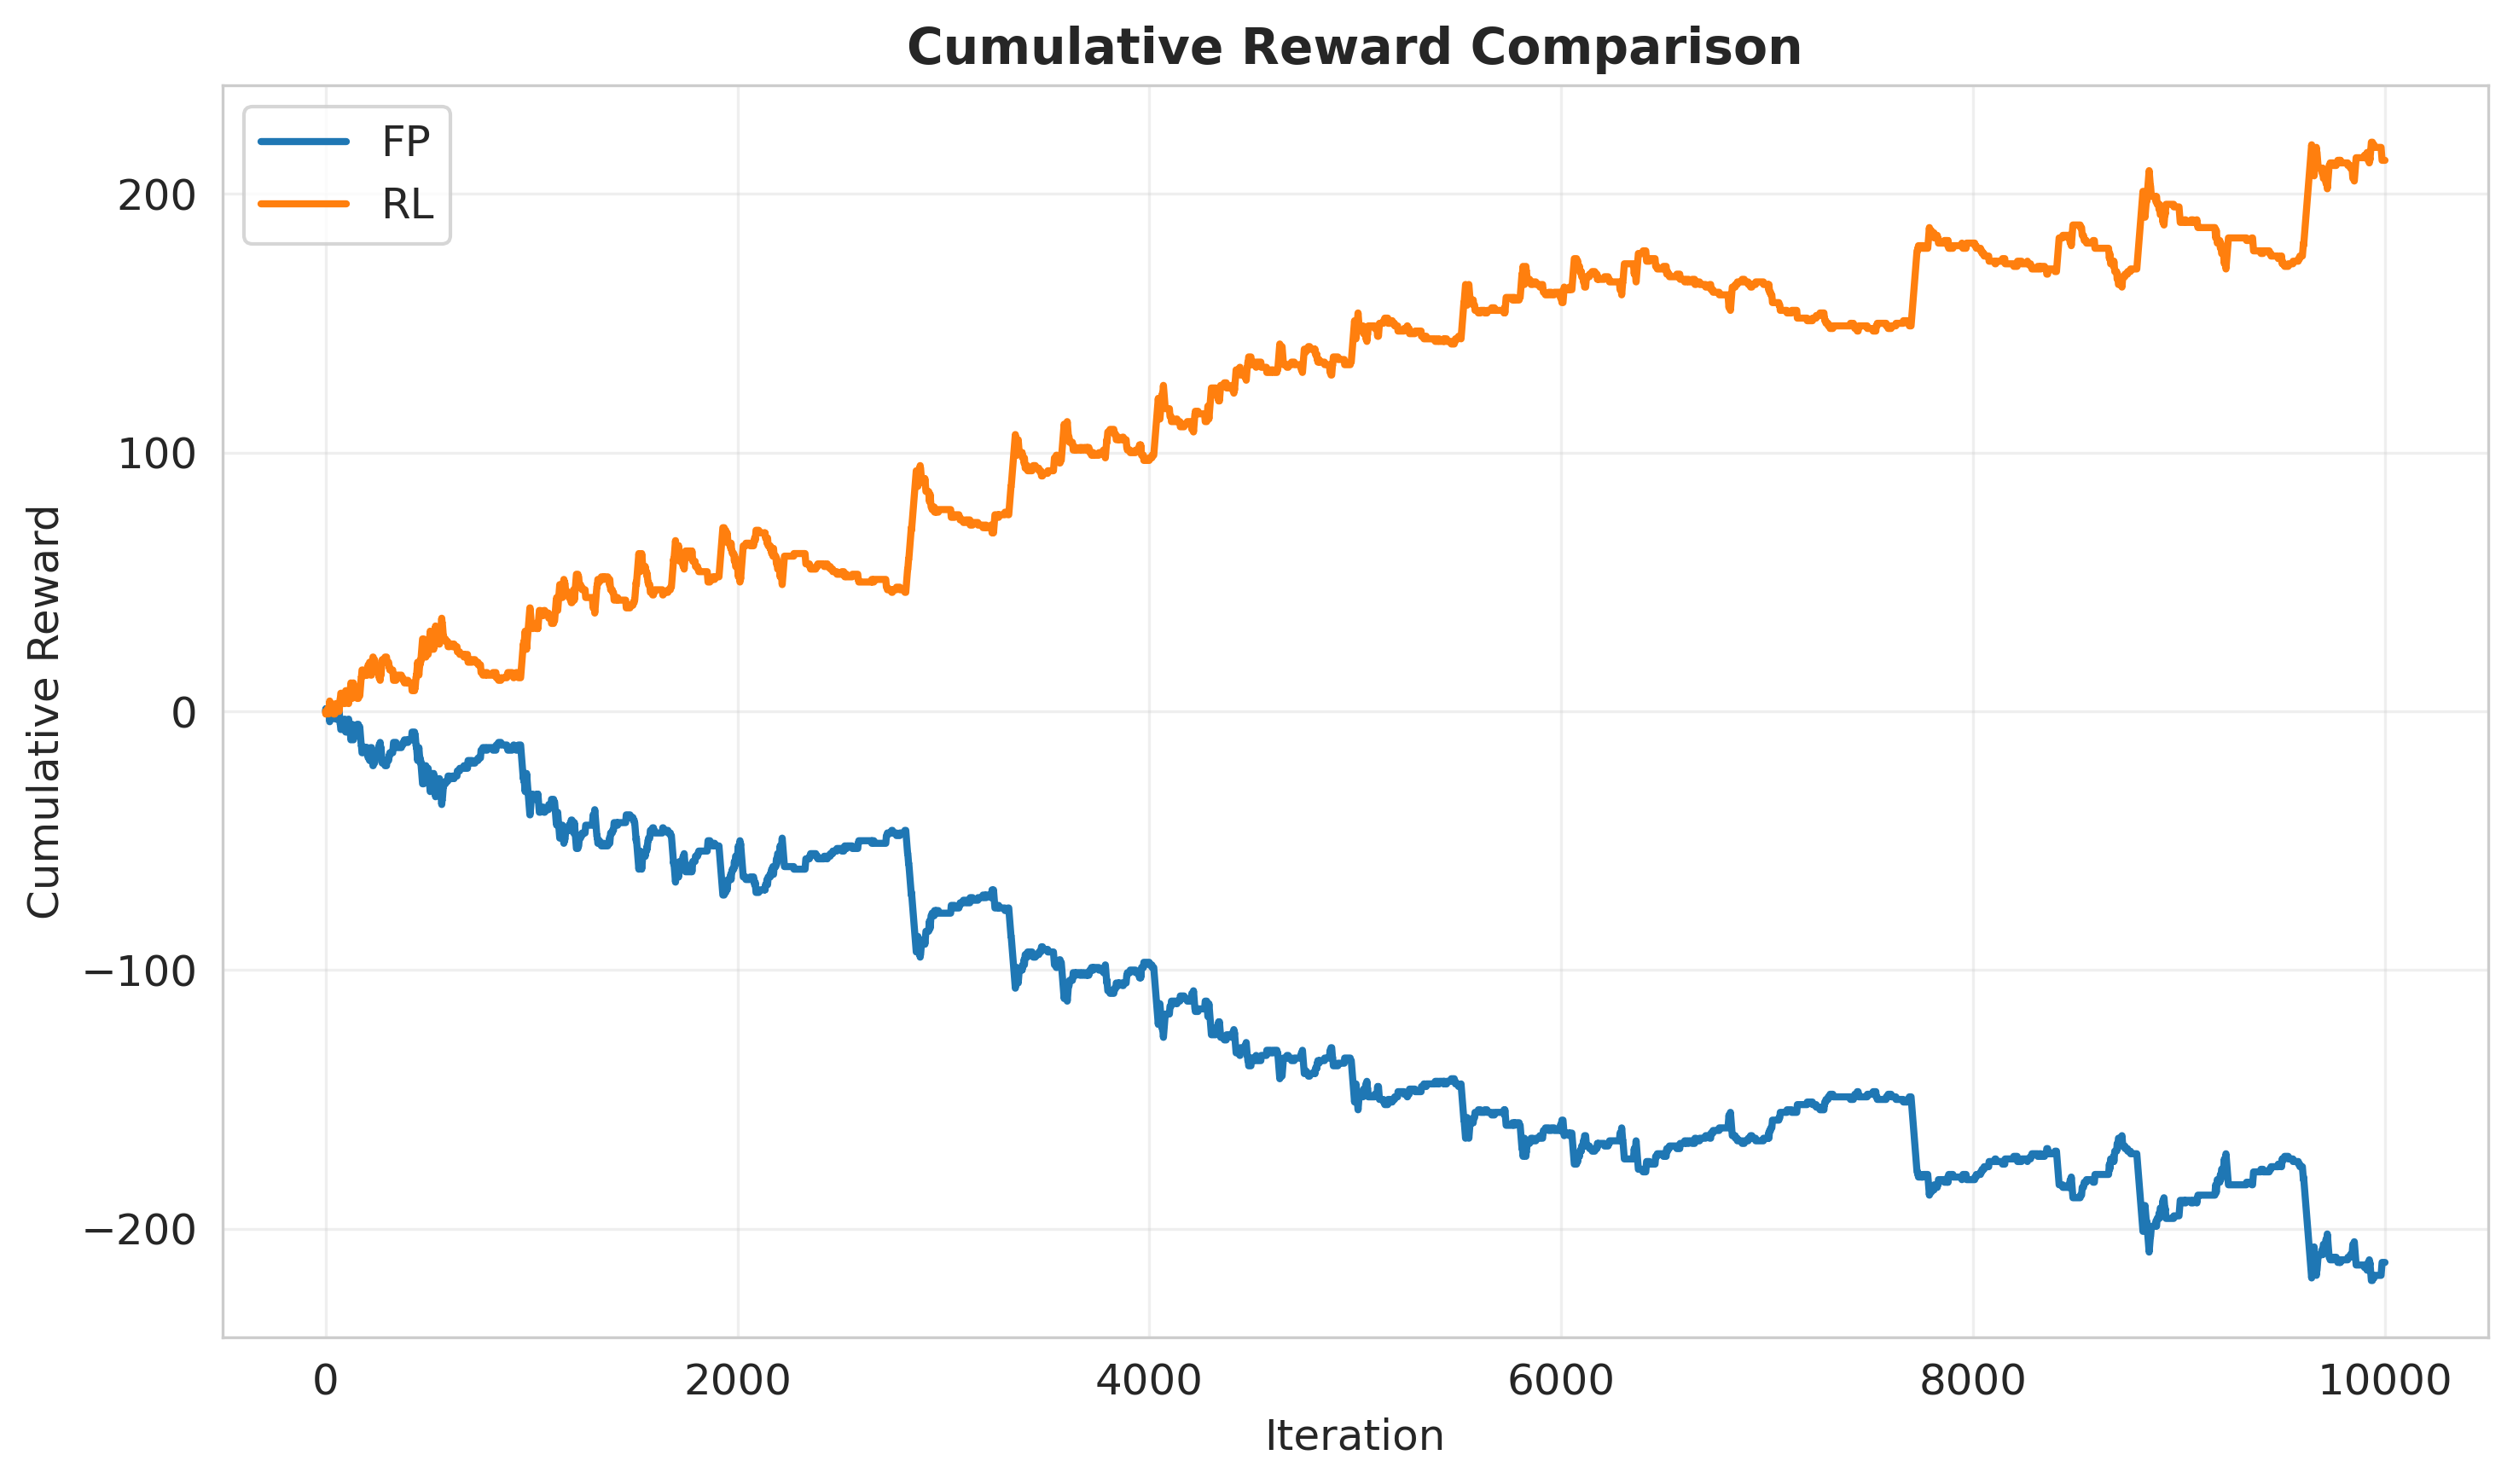
\includegraphics[width=0.8\textwidth]{../../results/plots/rock_paper_scissors/FP vs RL/reward_comparison.png}
\caption{Cumulative reward RPS. RL +213, FP −213.}
\end{figure}

\subsubsection{RL vs RL}

Αποτελέσματα: RL1 και RL2 distance 0.7670. RL1 cumulative +212, RL2 −212. Average +0.0212 / −0.0212.

Σε αντίθεση με το Matching Pennies RL vs RL (όπου τα rewards ήταν σχεδόν 0), εδώ υπάρχει ισχυρή ασυμμετρία (+212 vs −212). Αυτό υποδηλώνει κυκλική ή εκμεταλλευτική δυναμική: ένας RL agent πέτυχε να «προλάβει» τον άλλο και να συσσωρεύσει θετικό reward. Οι πολιτικές δεν σταθεροποιούνται στο (1/3, 1/3, 1/3) — η αστάθεια είναι πιο έντονη στο RPS λόγω του μεγαλύτερου χώρου ενεργειών (3×3). Αυτό είναι ουσιαστικό: εδώ η self-play δυναμική δεν «ισορροπεί» ούτε σε Nash ούτε σε συμμετρική κατανομή ανταμοιβών.

Εκτελέσαμε το ίδιο exploitability sweep και για το RPS (5.000 iterations ανά ζεύγος):

\begin{center}
\small
\begin{tabular}{@{}lccc@{}}
\toprule
 & \(\varepsilon=0.05\) & \(\varepsilon=0.10\) & \(\varepsilon=0.20\) \\
\midrule
\(\alpha=0.01\) & 0.9697 & 0.9393 & 0.8787 \\
\(\alpha=0.10\) & 0.9697 & 0.9393 & 0.8787 \\
\(\alpha=0.50\) & 0.9697 & 0.9393 & 0.8787 \\
\bottomrule
\end{tabular}
\end{center}

Οι τιμές (0.88--0.97) είναι χαμηλότερες από το Matching Pennies — το θεωρητικό μέγιστο στο RPS είναι περίπου 1.33 για καθαρή στρατηγική. Η ίδια μορφή επαναλαμβάνεται: η exploitability εξαρτάται μόνο από το \(\varepsilon\), όχι από το learning rate.

\begin{figure}[ht]
\centering
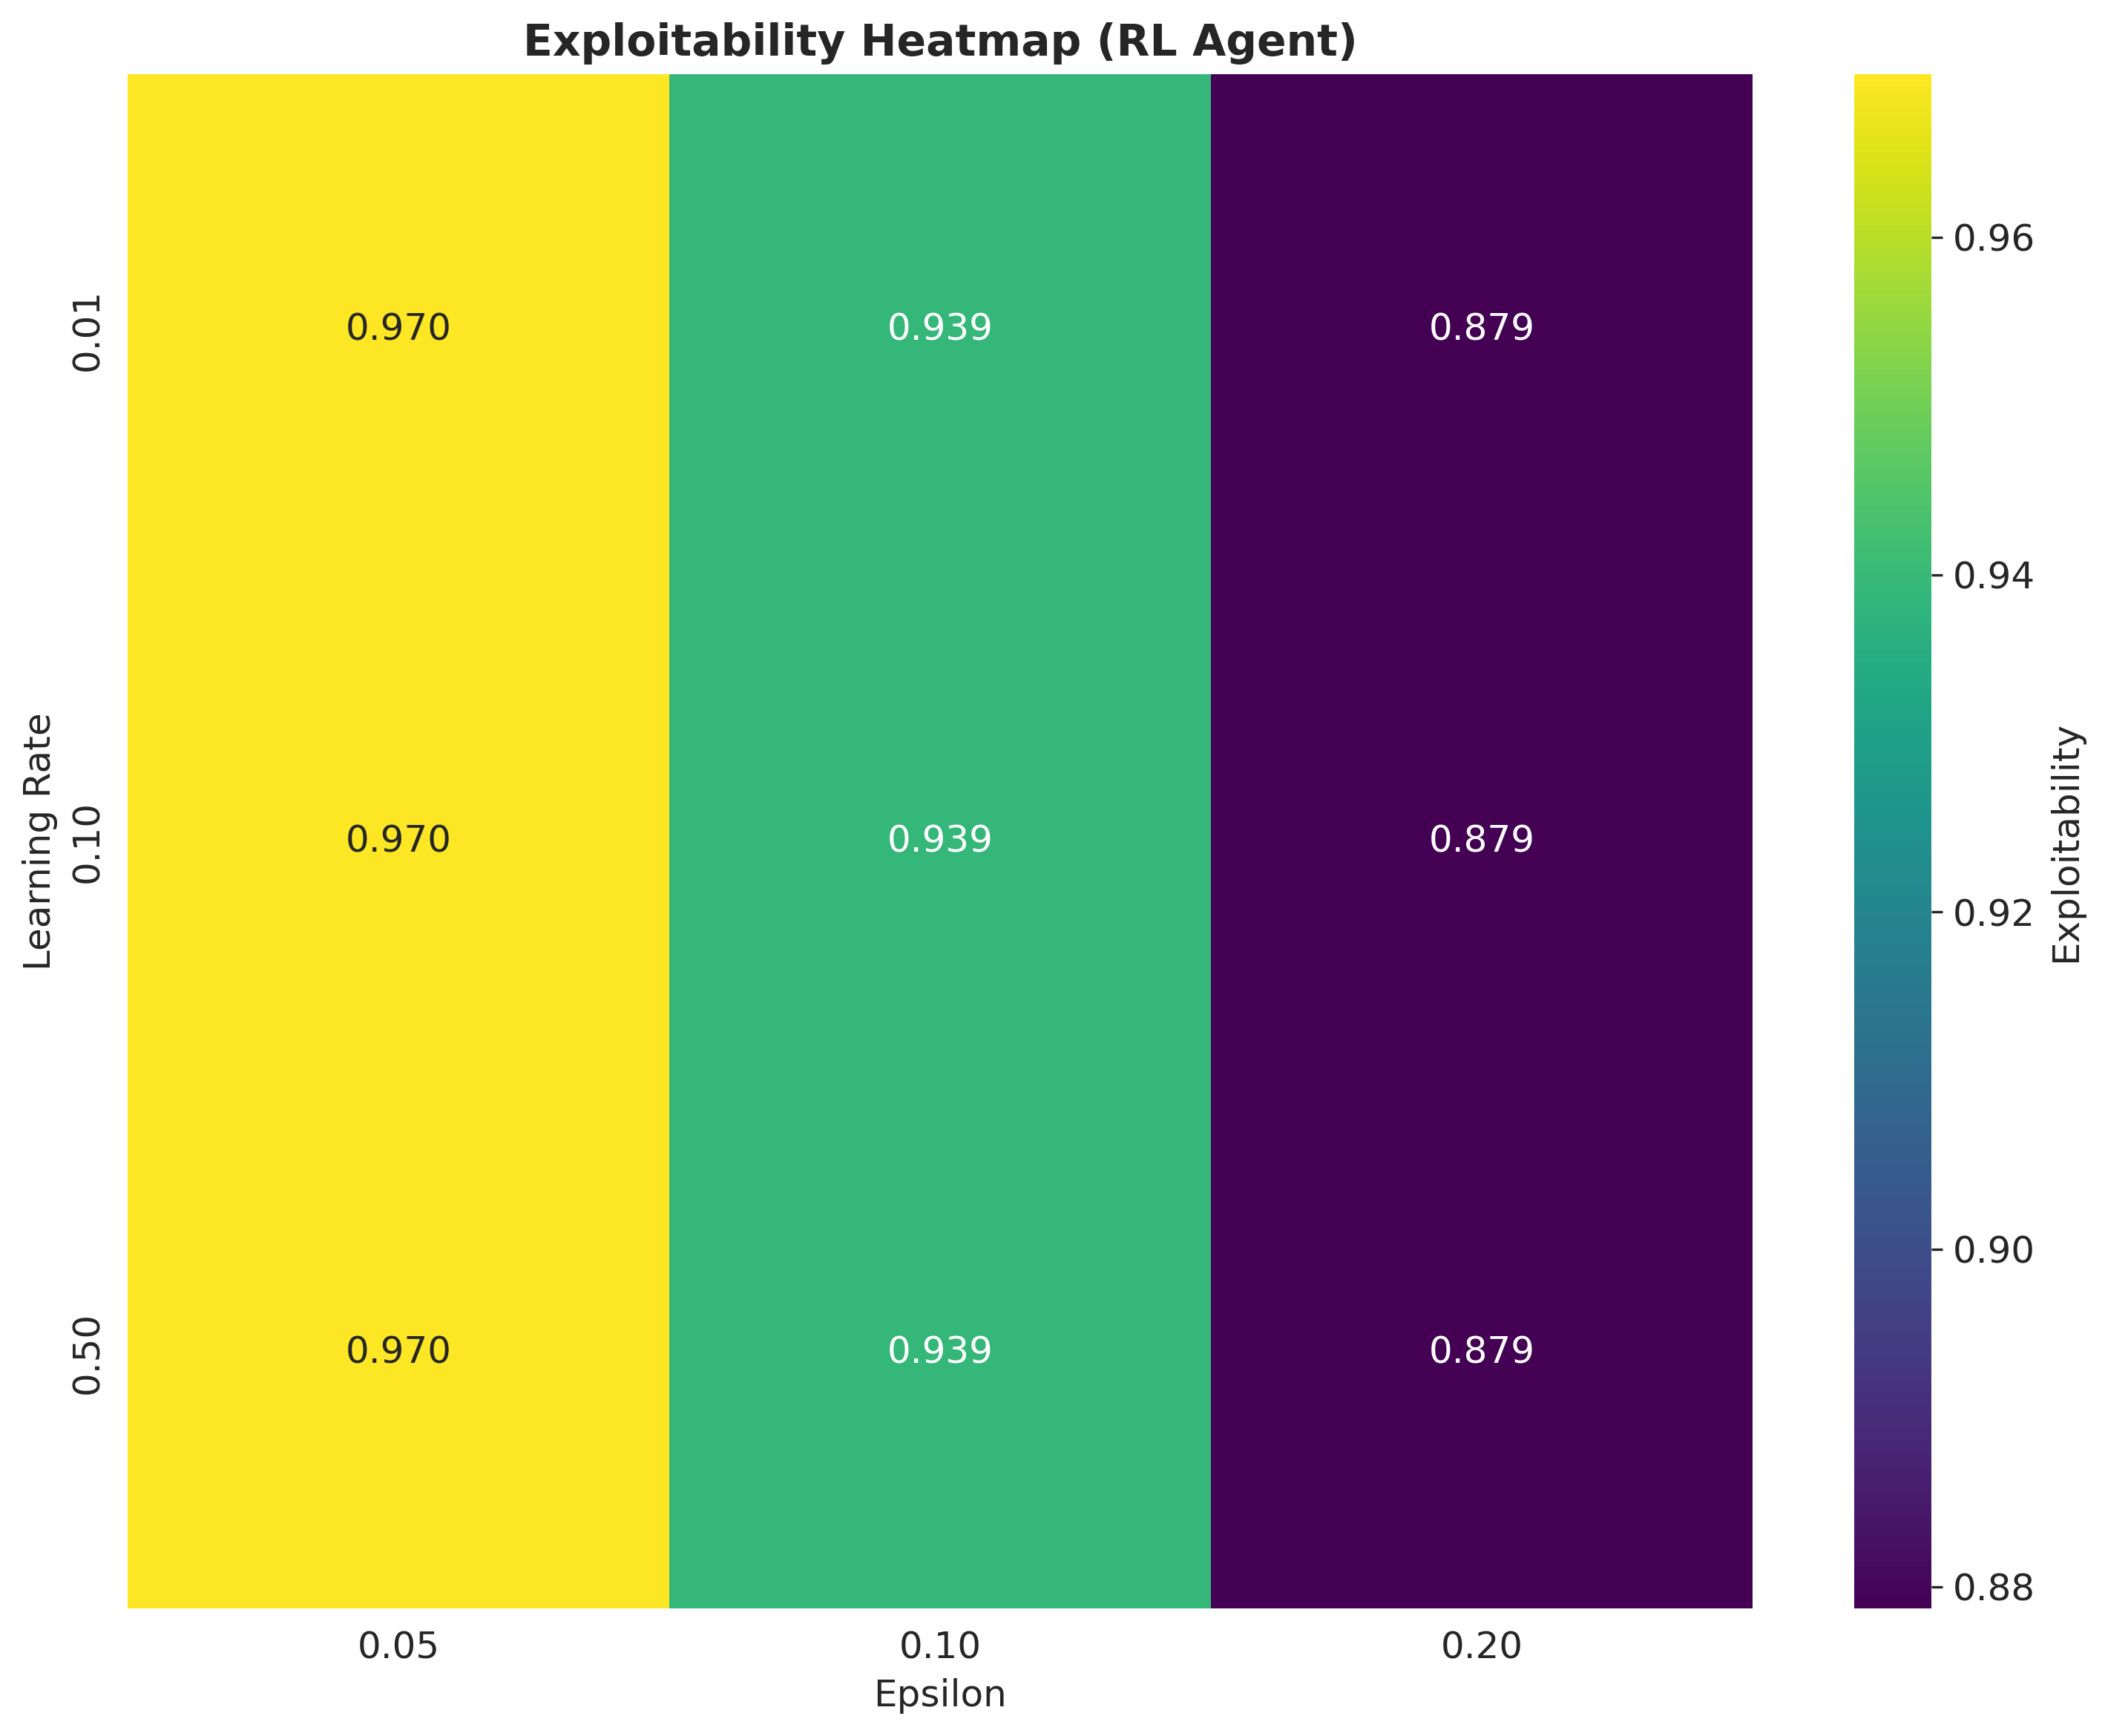
\includegraphics[width=0.8\textwidth]{../../results/plots/rock_paper_scissors/RL vs RL/exploitability_heatmap.png}
\caption{Exploitability heatmap στο Rock-Paper-Scissors (RL vs RL). Οι τιμές (0.88--0.97) είναι συμβατές με το μεγαλύτερο χώρο ενεργειών.}
\end{figure}

\subsection{Grid Game (Hunter–Prey, στοχαστικό, turn-based)}

Πλέγμα 3×3, max\_steps=20, 200.000 turns. Πηγές: \eng{results/plots/grid\_game/*/results.txt}. Συγκρίνουμε δύο ρεαλιστικά σεναρία: MinMax vs RL (Hunter = Minimax, Prey = Stochastic Q-Learning) και RL vs RL (και οι δύο Stochastic Q-Learning).

Εκτελέσαμε και τα δύο σεναρία σειράς κίνησης — πρώτος Hunter και πρώτο Prey — διότι σε πλέγμα τόσο μικρό (3×3) αν επαιζε πάντα πρώτος ο Hunter, το παίγνιο θα ήταν άδικο υπέρ του κυνηγού λόγω του μεγέθους του πίνακα. Οπότε τρέξαμε και τη διαφορετική σειρά (Prey πρώτο) ώστε να μελετήσουμε την επιρροή της σειράς κίνησης.

\subsubsection{MinMax vs RL}

\begin{center}
\resizebox{\textwidth}{!}{%
\small
\begin{tabular}{@{}lrrrrrr@{}}
\toprule
Πρώτος παίκτης & Episodes & Captures & Capture rate & Hunter total reward & Hunter mean reward & Prey \(\varepsilon\) \\
\midrule
Hunter & 10.264 & 670 & 6.5\% & +6.998,5 & +0.0698 & 0.068 \\
Prey & 10.282 & 682 & 6.6\% & −87.868,8 & −0.8787 & 0.068 \\
\bottomrule
\end{tabular}%
}
\end{center}

Hunter first: Ο Minimax Hunter έχει θετική συσσωρευμένη ανταμοιβή (+6.998,50) και capture rate 6.5\%. Το RL Prey μειώνει το epsilon (0.068) και μαθαίνει να αποφεύγει· ωστόσο το MinMax κυριαρχεί όταν κινείται πρώτος.

Prey first: Παρατηρούμε δραματική διαφορά. Το capture rate παραμένει παρόμοιο (6.6\%), αλλά το Hunter total reward είναι έντονα αρνητικό (−87.868,80). Αυτό οφείλεται στις timeout penalties: όταν το Prey κινείται πρώτο, έχει προτεραιότητα να διαφύγει· σε πολλά επεισόδια το παίγνιο φτάνει τα max\_steps χωρίς capture, ο Hunter λαμβάνει −10 ανά timeout και η συσσωρευμένη ζημιά υπερκαλύπτει τις captures (+10 έκαστη). Το RL Prey ωφελείται σημαντικά από τη σειρά κίνησης. Αυτό δείχνει ότι το capture rate είναι ανεπαρκές metric: η διαφορά οφείλεται στο πώς αλλάζει η κατανομή των τερματικών εκβάσεων και η συσσώρευση ποινών (timeouts/βήματα) όταν το Prey έχει το προβάδισμα της πρώτης κίνησης.

\subsubsection{RL vs RL}

\begin{center}
\small
\begin{tabular}{@{}lrrrrr@{}}
\toprule
Πρώτος παίκτης & Episodes & Captures & Capture rate & Hunter total reward & Hunter mean reward \\
\midrule
Hunter & 18.872 & 16.775 & 88.9\% & +230.170,7 & +2.1236 \\
Prey & 17.656 & 15.119 & 85.6\% & +177.072,6 & +1.7707 \\
\bottomrule
\end{tabular}
\end{center}

Στο RL vs RL το Hunter κυριαρχεί σε και τα δύο σεναρία. Capture rate 88.9\% (Hunter first) και 85.6\% (Prey first) — σημαντικά υψηλότερα από το MinMax vs RL (6.5–6.6\%). Ερμηνεία: όταν και οι δύο μαθαίνουν, ο RL Hunter μαθαίνει να κυνηγά πιο αποτελεσματικά, ενώ το RL Prey δεν μαθαίνει τόσο καλά να διαφεύγει όσο το Prey απέναντι σε MinMax. Στο MinMax vs RL, το RL Prey αντιμετωπίζει έναν «τέλειο» Hunter και ασκείται συστηματικά να διαφεύγει· στο RL vs RL και οι δύο εξελίσσονται ταυτόχρονα και η δυναμική οδηγεί σε υψηλή capture rate υπέρ του Hunter. Στο RL vs RL ο Hunter μαθαίνει πολύ ισχυρή πολιτική σύλληψης σε αυτό το μικρό state space. Η πρώτη κίνηση βοηθά το Prey, αλλά δεν αρκεί για να μετατρέψει το αποτέλεσμα σε «ισορροπημένη» κατάσταση: ο Hunter παραμένει σαφώς κυρίαρχος, κάτι που συνδέεται με το μικρό state space και τη δυναμότητα του Q-learning να μάθει γρήγορα αποτελεσματικές chasing πολιτικές.

\begin{figure}[ht]
\centering
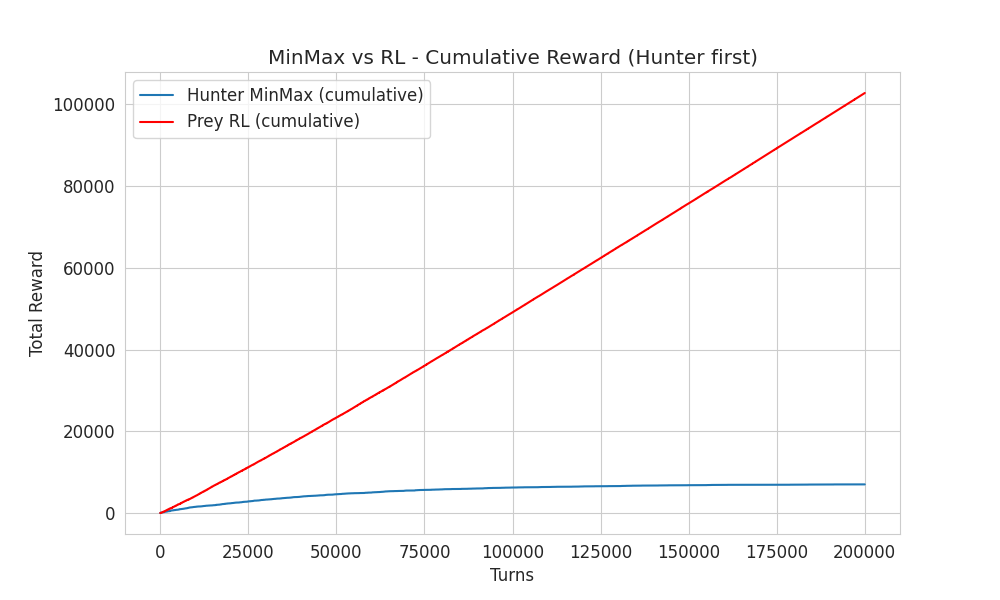
\includegraphics[width=0.8\textwidth]{../../results/plots/grid_game/MinMax vs RL - Hunter first/cumulative_reward.png}
\caption{Συσσωρευμένο reward στο MinMax vs RL (Hunter first). Hunter (Minimax) θετική τάση.}
\end{figure}

\begin{figure}[ht]
\centering
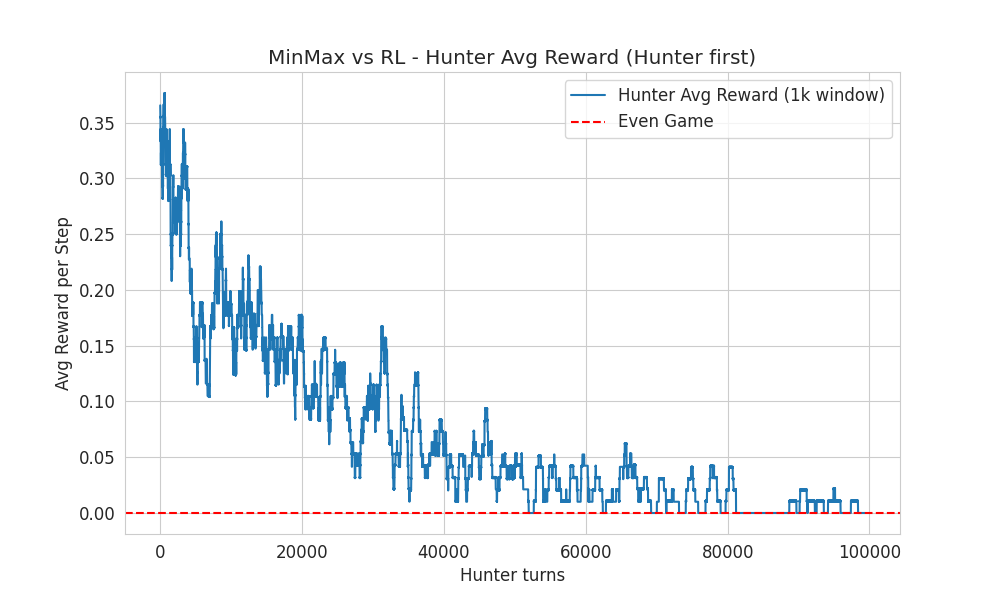
\includegraphics[width=0.8\textwidth]{../../results/plots/grid_game/MinMax vs RL - Hunter first/avg_reward.png}
\caption{Μέσο reward (κινητός μέσος) — Hunter first. Ο Hunter έχει θετικό μέσο reward· το Prey βελτιώνεται με το χρόνο.}
\end{figure}

\begin{figure}[ht]
\centering
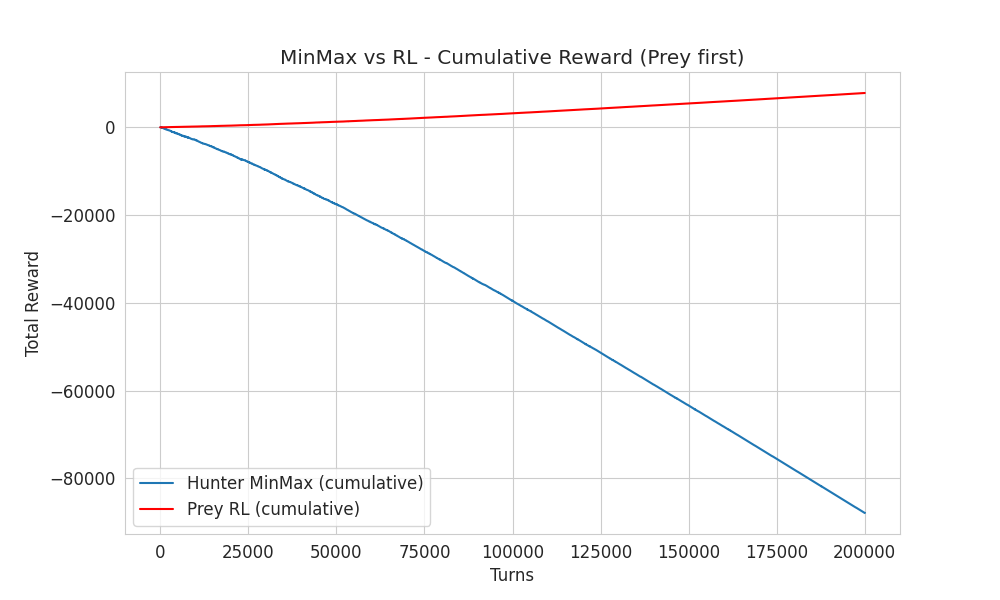
\includegraphics[width=0.8\textwidth]{../../results/plots/grid_game/MinMax vs RL - Prey first/cumulative_reward.png}
\caption{Συσσωρευμένο reward στο MinMax vs RL (Prey first). Ο Hunter λαμβάνει αρνητικό reward λόγω timeout penalties.}
\end{figure}

Συμπέρασμα Grid Game: (1) Η σειρά κίνησης επηρεάζει δραστικά το MinMax vs RL· Prey first → πολλά timeouts → αρνητικό Hunter reward παρά παρόμοιο capture rate. (2) Στο RL vs RL ο Hunter κυριαρχεί (85–89\% capture)· όταν και οι δύο μαθαίνουν, η μάθηση του Hunter να κυνηγά υπερνικά την ικανότητα του Prey να διαφεύγει. (3) Το MinMax Hunter (6.5\% capture vs RL Prey) είναι αξιοπρεπές αλλά το RL Prey μαθαίνει να διαφεύγει· αντίθετα, το RL Prey vs RL Hunter είναι πιο ευάλωτο. Όταν περνάμε από στατικά matrix games σε στοχαστικά/διαδοχικά παιχνίδια, η έννοια «λύση» μετασχηματίζεται από «μικτή στρατηγική» σε «state-dependent policy» και τα metrics πρέπει να ακολουθήσουν. Το Grid Hunter-Prey ανέδειξε ότι ένα προφανές metric όπως το capture rate μπορεί να αποτυγχάνει να περιγράψει την απόδοση. Η σειρά κίνησης μπορεί να αφήνει το capture rate σχεδόν αμετάβλητο αλλά να αντιστρέψει πλήρως το συνολικό reward λόγω timeout/step penalties. Αυτό είναι γενικό μάθημα για evaluation: στα sequential games πρέπει να κοιτάμε (α) ποσοστά επιτυχίας, (β) χρόνο μέχρι τερματισμό, (γ) κατανομή τερματικών εκβάσεων, και (δ) συνολικό reward, γιατί το reward είναι ευαίσθητο στη διαδρομή, όχι μόνο στο τελικό γεγονός.

% ========== ΚΕΦΑΛΑΙΟ 4 ==========
\section{Συμπεράσματα από τα Πειράματα}

Σύγκλιση στο Nash και FP: Σε FP vs FP (Matching Pennies και RPS) οι τελικές αποστάσεις από το Nash είναι πολύ μικρές (0.0007, 0.0092 στο MP· 0.0032 και στα δύο στο RPS) και τα cumulative rewards κοντά στο μηδέν. Αυτό επιβεβαιώνει ότι η Fictitious Play συγκλίνει προς το mixed Nash σε zero-sum matrix games όταν και οι δύο παίκτες τη χρησιμοποιούν. Η λέξη «ισορροπία» έχει πολύ συγκεκριμένο νόημα στα zero-sum matrix games· εκεί οφείλεις να αξιολογείς με μέτρο που συνδέεται με Nash/minimax. Με αυτό το κριτήριο, το FP σε self-play λειτουργεί όπως περιμένουμε. Αυτό δεν σημαίνει ότι οι καθαρές κινήσεις σταματούν να ταλαντώνονται, αλλά σημαίνει ότι η μακροχρόνια στατιστική συμπεριφορά προσεγγίζει τη mixed equilibrium. Αν ο στόχος της εφαρμογής ήταν «να βρω/προσεγγίσω mixed Nash σε repeated zero-sum», το FP είναι η πιο άμεση και ερμηνεύσιμη επιλογή από τις δύο.

Εκμετάλλευση FP από RL: Σε FP vs RL, στα δύο παίγνια η FP παραμένει κοντά στο Nash (απόσταση 0 ή 0.0152) αλλά ο RL έχει μεγάλη απόσταση (0.6642, 0.7670) και σημαντικά μεγαλύτερο cumulative reward (MP: +374 vs −374· RPS: +213 vs −213). Το RL δεν συγκλίνει στο NE αλλά μαθαίνει να παίζει best response στις εμπειρικές συχνότητες της FP. Αυτό φαίνεται και από το external regret: η FP έχει υψηλό θετικό regret (388, 234), ενώ ο RL έχει αρνητικό ή σχεδόν μηδενικό (−374, −3) — η FP δεν είναι no-regret απέναντι σε προσαρμοστικούς αντιπάλους. Η απόσταση από Nash και η απόδοση σε reward σε πεπερασμένο ορίζοντα δεν ταυτίζονται, και μάλιστα μπορούν να συγκρουστούν έντονα. Η σωστή ερμηνεία δεν είναι ότι «η Nash είναι λάθος», ούτε ότι «το FP είναι κακό». Είναι ότι η Nash είναι έννοια ασφάλειας απέναντι σε βέλτιστο (equilibrium) αντίπαλο, ενώ εδώ ο αντίπαλος είναι μαθησιακός και μη-στατικός. Το RL προσαρμόζεται σε αυτή τη μη-στασιμότητα και μπορεί να αξιοποιήσει προσωρινές και τοπικές κανονικότητες της δυναμικής του FP. Άρα, όταν ο αντίπαλος είναι adaptive, το να παίζεις «ισορροπιακά» δεν εγγυάται καλύτερη απόδοση στο training horizon.

RL vs RL και αστάθεια (matrix games): Το απλό tabular Q-learning δεν είναι, από μόνο του, μέθοδος υπολογισμού Nash σε matrix games. Τα πειράματα RL vs RL το δείχνουν ξεκάθαρα: και στις δύο περιπτώσεις οι τελικές αποστάσεις από Nash είναι μεγάλες. Επιπλέον, στο RPS εμφανίζεται έντονη ασυμμετρία rewards σε self-play. Στο RL vs RL οι αποστάσεις παραμένουν υψηλές (0.6642 στο MP, 0.7670 στο RPS). Τα cumulative rewards είναι είτε σχεδόν μηδέν (MP: ±4) είτε μεγάλα και αντίθετα (RPS: +212 vs −212). Το περιβάλλον είναι non-stationary και το απλό Q-learning δεν συγκλίνει σε σταθερή ισορροπία. Αυτό σημαίνει ότι η self-play δυναμική δεν «κλειδώνει» σε ισορροπία, αλλά μπορεί να οδηγήσει σε καταστάσεις που διατηρούν πλεονέκτημα για έναν παίκτη στο συγκεκριμένο trajectory. Η διαφορά MP vs RPS: στο RPS η κυκλική δυναμική οδηγεί σε ισχυρή ασυμμετρία· στο MP κανένας δεν προλαβαίνει τον άλλο. Αν το ζητούμενο ήταν equilibrium computation με RL, θα χρειαζόταν διαφορετική κατηγορία αλγορίθμων (π.χ. minimax-Q ή explicit equilibrium-driven updates), όχι plain Q-learning.

No-regret και απόδοση: Όταν ο RL αντιμετωπίζει FP, έχει αρνητικό regret και υψηλό cumulative reward· η FP έχει γραμμικά αυξανόμενο regret. Η απόδοση (cumulative reward) ευνοεί τον πράκτορα που προσαρμόζεται (RL) έναντι του που συγκλίνει στο Nash αλλά μένει προβλέψιμος (FP).

MinMax vs RL στο Grid: Ο Hunter με Minimax (βάθος 4) πετυχαίνει capture rate 6.5–6.6\% απέναντι σε RL Prey. Όταν κινείται πρώτος έχει θετικό reward (+6.998,5)· όταν το Prey κινείται πρώτο η συσσωρευμένη ζημιά από timeouts (−87.868,8) υπερκαλύπτει τις captures. Το RL Prey μαθαίνει να διαφεύγει αποτελεσματικά από τον MinMax Hunter.

RL vs RL στο Grid: Σημαντική διαφορά: capture rate 85–89\% — πολύ υψηλότερο από το MinMax vs RL (6.5–6.6\%). Όταν και οι δύο μαθαίνουν, ο RL Hunter μαθαίνει να κυνηγά πιο αποτελεσματικά από ότι το RL Prey μαθαίνει να διαφεύγει. Σε μικρά state spaces το tabular Q-learning μπορεί να είναι εξαιρετικά αποτελεσματικό στην παραγωγή ισχυρών πολιτικών — φαίνεται από τα 85–89\% capture rates του Hunter στο RL vs RL grid. Αυτό δεν αναιρεί τα προβλήματα της multiagent non-stationarity στα matrix games· δείχνει ότι όταν το πρόβλημα έχει δομή τύπου MDP/Markov game και υπάρχει επαρκής επανάληψη, το Q-learning μπορεί να συγκλίνει πρακτικά σε υψηλής ποιότητας πολιτικές. Η επιτυχία αυτή είναι συνδεδεμένη με το μέγεθος του state space, τη διαμόρφωση ανταμοιβών και το exploration schedule. Αντίθετα με το MinMax vs RL, όπου το RL Prey αντιμετωπίζει «τέλειο» αντίπαλο και ασκείται στη διαφυγή, στο RL vs RL η συμπρωτεύουσα εξέλιξη οδηγεί σε κυριαρχία του Hunter.

Συνολικά: Το FP και το Q-learning δεν είναι «ανταγωνιστές» που συγκρίνονται με μία μόνο λέξη τύπου «καλύτερο». Είναι εργαλεία με διαφορετικό στόχο. Το FP είναι ευθυγραμμισμένο με equilibrium reasoning σε repeated matrix games και αποδίδει εκεί με τρόπο που μετριέται καθαρά με distance-to-Nash. Το Q-learning είναι ευθυγραμμισμένο με policy optimization σε sequential περιβάλλοντα και αποδίδει ιδιαίτερα καλά στο grid, ενώ σε matrix games μπορεί να κερδίζει απέναντι σε FP χωρίς να παίζει καθόλου ισορροπιακά και χωρίς να εμφανίζει σύγκλιση σε Nash σε self-play. Το βασικό επιστημονικό συμπέρασμα από το σύνολο των πειραμάτων είναι ότι η επιλογή μεθόδου πρέπει να γίνεται με βάση το ζητούμενο: equilibrium computation, robust ασφαλής συμπεριφορά (minimax), ή πρακτική βελτιστοποίηση απόδοσης σε δυναμικό περιβάλλον, καθώς και με βάση το αν το παιχνίδι είναι στατικό ή διαδοχικό/στοχαστικό. Η μελέτη δείχνει ξεκάθαρα τη διαφορά μεταξύ αλγορίθμων που στοχεύουν στη σύγκλιση στο Nash (FP) και αλγορίθμων που μεγιστοποιούν reward απέναντι σε προσαρμοστικούς αντιπάλους (RL). Τα δεδομένα από όλα τα \eng{results.txt} και τα plots τεκμηριώνουν αυτά τα συμπεράσματα. Η εργασία παραμένει στο πλαίσιο απλών προβλημάτων, ώστε η βαθιά κατανόηση και η ξεκάθαρη απεικόνιση δυνατοτήτων και αδυναμιών των αλγορίθμων να μην θυσιάζονται σε περιττή πολυπλοκότητα.

\end{document}
